\documentclass{article}

\usepackage[main, final]{neurips_2026}

\makeatletter
\renewcommand{\@toptitlebar}{\vskip 0.25in \vskip -\parskip}
\renewcommand{\@bottomtitlebar}{\vskip 0.29in \vskip -\parskip \vskip 0.09in}
\makeatother

\usepackage[utf8]{inputenc}
\usepackage[T1]{fontenc}
\usepackage{hyperref}
\usepackage{url}
\usepackage{booktabs}
\usepackage{amsfonts}
\usepackage{nicefrac}
\usepackage{microtype}
\usepackage{xcolor}
\usepackage{array}
\usepackage{ragged2e}
\usepackage{graphicx}
\usepackage{float}
\usepackage{titlesec}
\usepackage{amsmath}

\titleformat{\section}{\normalfont\LARGE\bfseries}{\thesection}{0.5em}{}
\titleformat{\subsection}{\normalfont\Large\bfseries}{\thesubsection}{0.5em}{}
\titleformat{\subsubsection}{\normalfont\large\bfseries}{\thesubsubsection}{0.5em}{}


\begin{document}
\maketitle

\section*{6. Dimensionality Reduction}
\label{sec:q6}

This section asks whether taxi trips fall into natural types. It uses the cleaned data from Section 1 (1{,}442{,}031 trips) and the airport flag from Section 5 (pickup or drop-off within 2\,km of JFK or Newark). We reduce the data with PCA, t-SNE~\hyperref[ref:2]{[2]} and UMAP~\hyperref[ref:3]{[3]}, and cluster with DBSCAN~\hyperref[ref:1]{[1]}. All random steps use seed 42.

\subsection*{6.1 Feature matrix}

A random sample of 20{,}000 cleaned trips was drawn with \texttt{random\_state=42}. It contains 598 airport trips (3.0\%) and 28.5\% weekend trips, close to the shares in the full cleaned data. Table~\ref{tab:q6_features} lists the eleven features.

\begin{table}[!htbp]
  \caption{Features used for dimensionality reduction. All columns are standardised to zero mean and unit variance after the transform shown.}
  \label{tab:q6_features}
  \centering
  \small
  \begin{tabular}{lll}
    \toprule
    Group & Columns & Transform \\
    \midrule
    Location & pickup/drop-off latitude and longitude & none \\
    Trip size & distance (km), duration (s) & $\log(1+x)$ \\
    Trip pace & average speed (km/h) & none \\
    Time of day & pickup hour $h$ & $\sin(2\pi h/24)$, $\cos(2\pi h/24)$ \\
    Day of week & pickup day $d$ (Mon $=0$) & $\sin(2\pi d/7)$, $\cos(2\pi d/7)$ \\
    \bottomrule
  \end{tabular}
\end{table}

\textbf{Features.} The four coordinates say where a trip happens. Distance, duration and speed say what kind of trip it is. Hour and day say when it happens. Together they cover the dimensions along which trip "types" (commutes, airport runs, late-night rides) would differ.

\textbf{Encoding.} Hour and day are cyclic: 23:00 is one hour from 00:00, and Sunday is next to Monday. Encoding them as an integer would place these neighbours at opposite ends of a line. The sine/cosine pair puts them on a circle instead.

\textbf{Skew and scaling.} Distance and duration are strongly right-skewed (skewness 2.79 and 2.46), so a few long airport trips would dominate a variance-based method. After $\log(1+x)$ their skewness falls to 0.96 and $-0.20$. Speed is only moderately skewed (1.46) and was left linear on purpose: $\log(\text{speed}) = \log(\text{distance}) - \log(\text{duration}) + c$, so a logged speed would be an almost exact linear combination of the other two columns. The features also have very different units (degrees with a standard deviation near $0.03$, seconds in the hundreds). PCA, t-SNE and UMAP all work with Euclidean distances, so unscaled data would be dominated by duration. Standard scaling gives each column the same weight. We chose it over min--max scaling because the coordinates contain a few far-away airport points that would compress everyone else into a narrow range.

The scaled matrix and the sample ids were saved as \texttt{q6\_feature\_matrix.csv} and \texttt{q6\_sample\_ids.csv}, so that every embedding in this section is computed on exactly the same trips.

\subsection*{6.2 PCA}

\begin{figure}[!htbp]
  \centering
  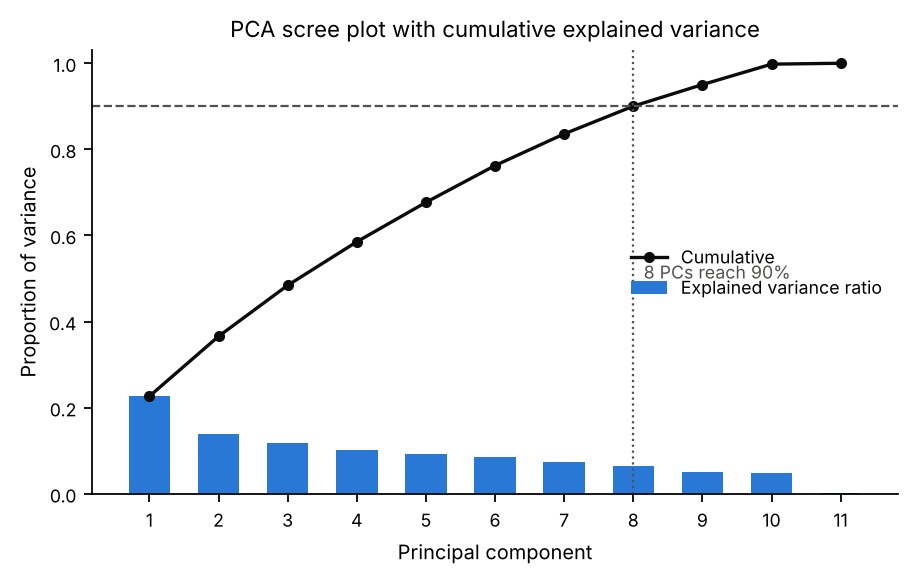
\includegraphics[width=0.53\linewidth]{section6_plots/q6_2_scree.png}\hfill
  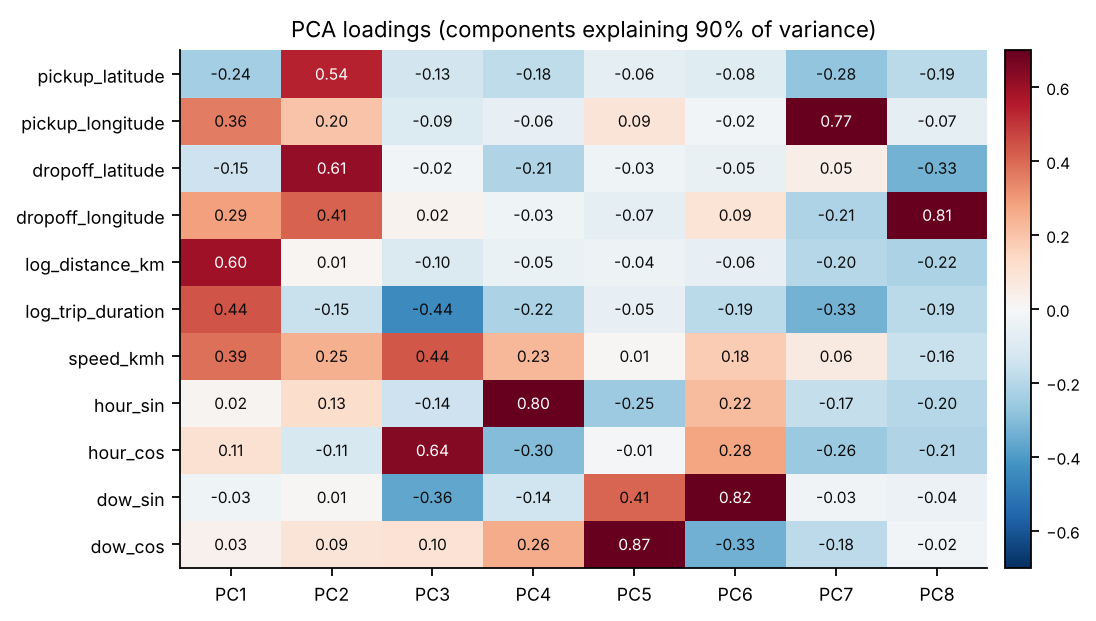
\includegraphics[width=0.45\linewidth]{section6_plots/q6_2_loadings.png}
  \caption{Left: explained variance per component and cumulative variance. Right: loadings of the eight components needed for 90\% of the variance.}
  \label{fig:q6_scree}
\end{figure}

The variance is spread thinly (Figure~\ref{fig:q6_scree}). PC1 explains 22.7\% and PC2 13.9\%, and \textbf{eight of the eleven components are needed to reach 90\%} (90.0\%). The features are only weakly correlated, so a linear projection cannot compress them much. The last component explains just 0.2\%: it is the near-dependency between log distance, log duration and speed.

\textbf{Loadings.} PC1 is a \emph{trip length} axis. Log distance ($0.60$), log duration ($0.44$) and speed ($0.39$) load positively, together with pickup and drop-off longitude ($0.36$, $0.29$). High PC1 therefore means long, fast trips heading east out of Manhattan. PC2 is a \emph{north--south location} axis: drop-off and pickup latitude load at $0.61$ and $0.54$, separating uptown trips from downtown and Brooklyn trips. The time features barely appear in PC1 or PC2. Hour loads on PC3 and PC4 ($\cos$: $0.64$; $\sin$: $0.80$) and day of week on PC5 and PC6 ($\cos$: $0.87$; $\sin$: $0.82$).

\begin{figure}[!htbp]
  \centering
  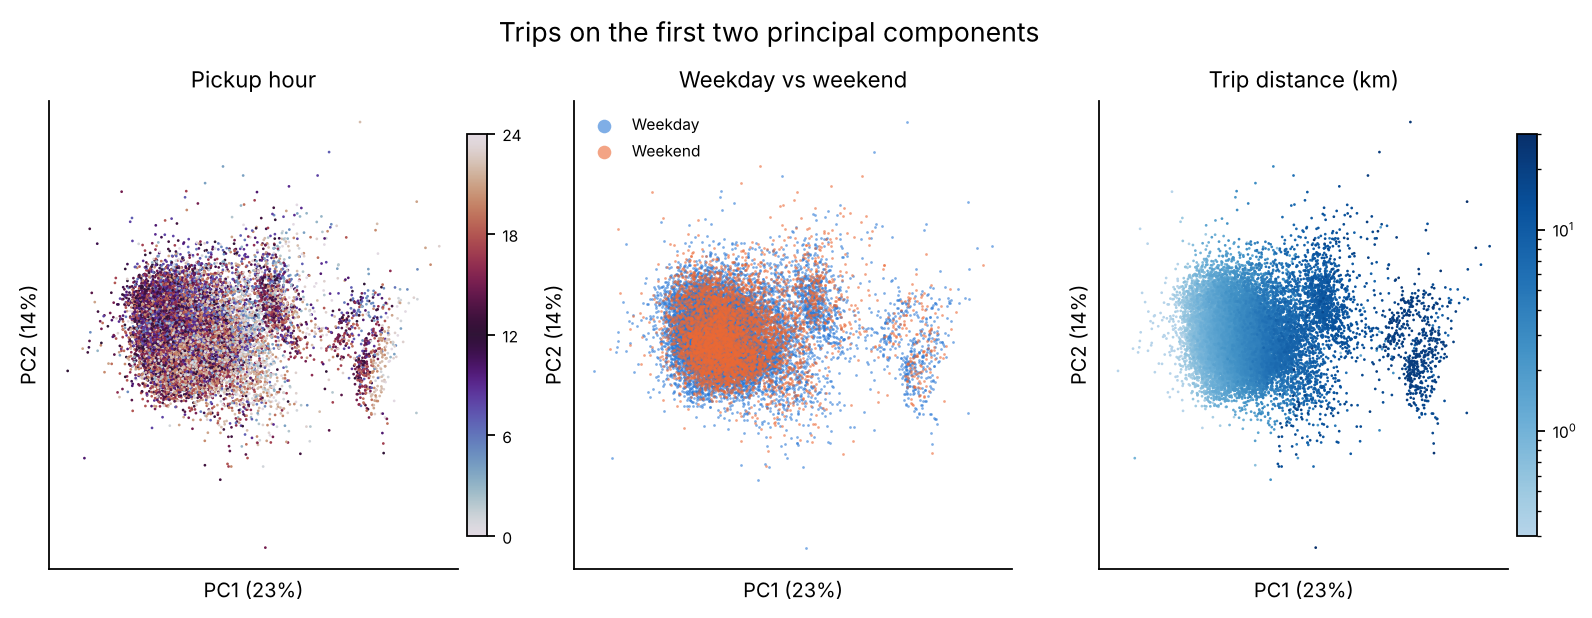
\includegraphics[width=0.85\linewidth]{section6_plots/q6_2_pca_pc1_pc2.png}
  \caption{Trips on PC1 and PC2, coloured by pickup hour, weekday/weekend and trip distance (log colour scale).}
  \label{fig:q6_pca}
\end{figure}

Figure~\ref{fig:q6_pca} confirms this reading. Distance increases smoothly from left to right, and the airport runs form a separate band on the far right. Hour and weekday/weekend show no pattern on these two axes, because that information sits on PC3--PC6. Apart from the airport band, the trips form one continuous cloud.

\subsection*{6.3 t-SNE}

\begin{figure}[!htbp]
  \centering
  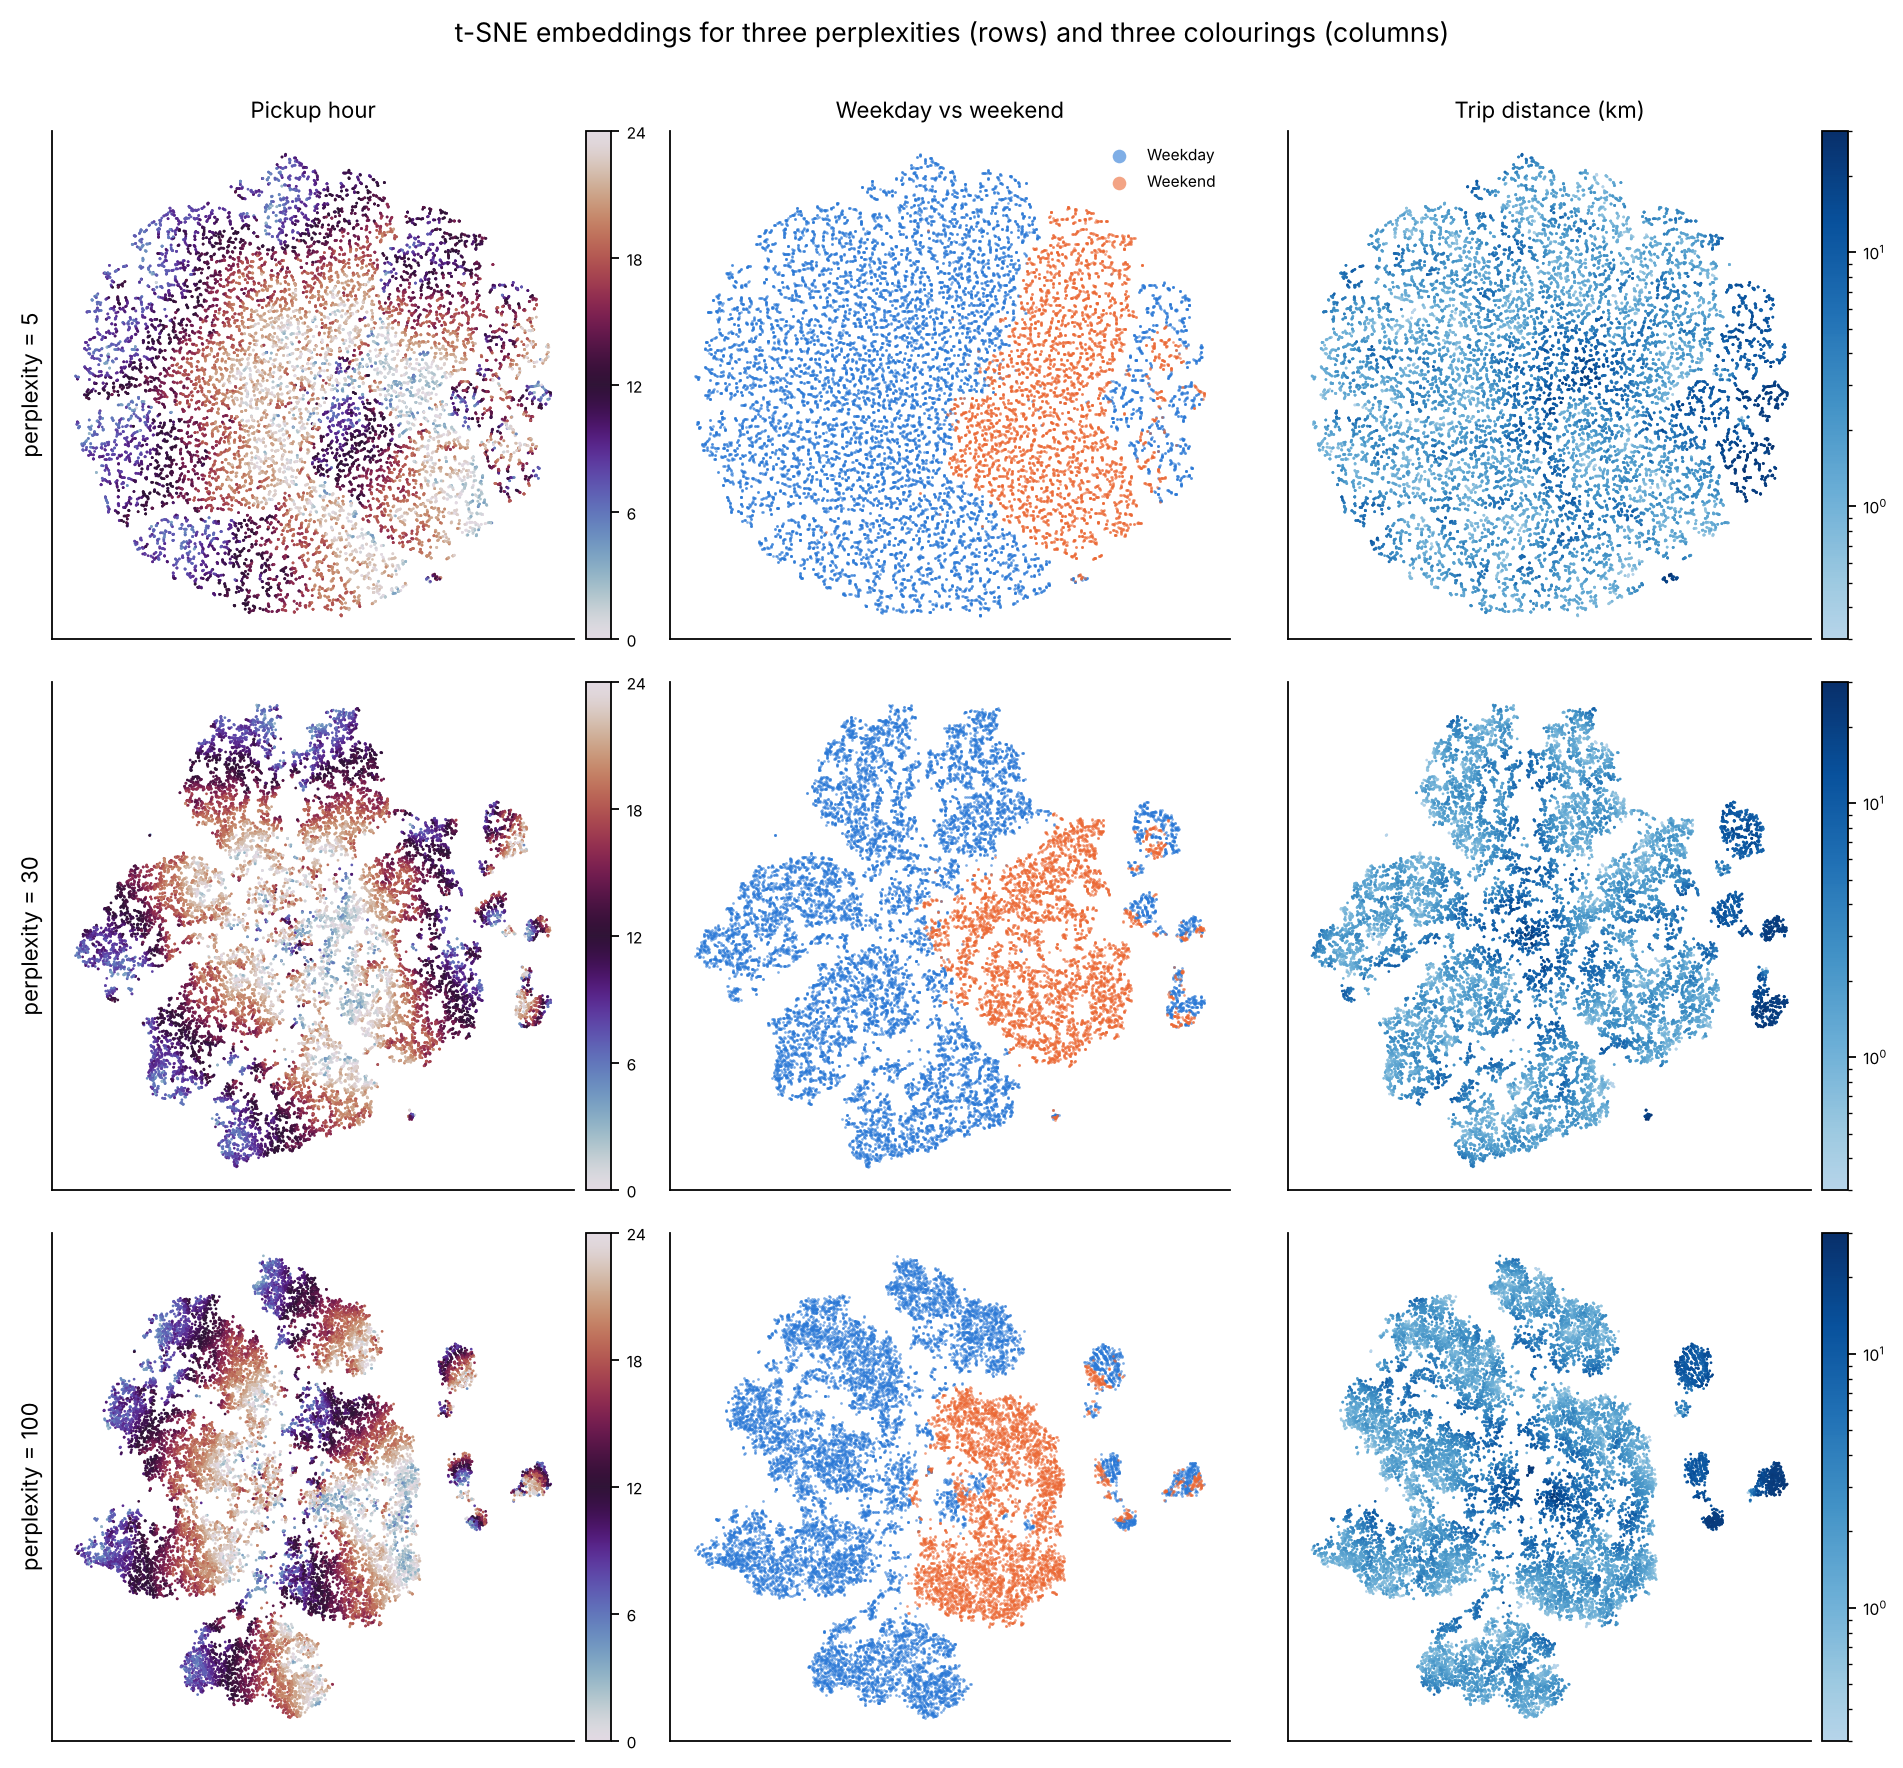
\includegraphics[width=0.7\linewidth]{section6_plots/q6_3_tsne_grid.png}
  \caption{t-SNE embeddings (\texttt{init="pca"}) for perplexity 5, 30 and 100 (rows), coloured by pickup hour, weekday/weekend and distance (columns).}
  \label{fig:q6_tsne}
\end{figure}

In t-SNE, perplexity sets the effective number of neighbours each point tries to keep close~\hyperref[ref:2]{[2]} (Figure~\ref{fig:q6_tsne}). At \textbf{perplexity 5} the embedding is a single disc of short strands. Neighbourhoods are tiny, so only very local similarity survives, and the only visible split is between weekday and weekend trips. At \textbf{perplexity 30} the disc breaks into lobes, and small separate islands of long trips appear on the right. At \textbf{perplexity 100} the lobes become compact, weekday and weekend occupy clearly different regions, and the long-trip islands (airport and LaGuardia runs) are cleanly separated. Within each lobe the hour colouring runs as a smooth gradient from morning to night, so t-SNE arranges time of day \emph{inside} the groups rather than splitting on it.

Larger perplexity therefore gives coarser, more global structure but costs more time (86\,s, 112\,s and 161\,s). Measured on a fixed subset of 3{,}000 trips, trustworthiness at $k=15$ rises from 0.943 to 0.978 and the correlation of pairwise distances with the original space from 0.295 to 0.357 (Table~\ref{tab:q6_scores}).

\subsection*{6.4 UMAP}

\begin{figure}[!htbp]
  \centering
  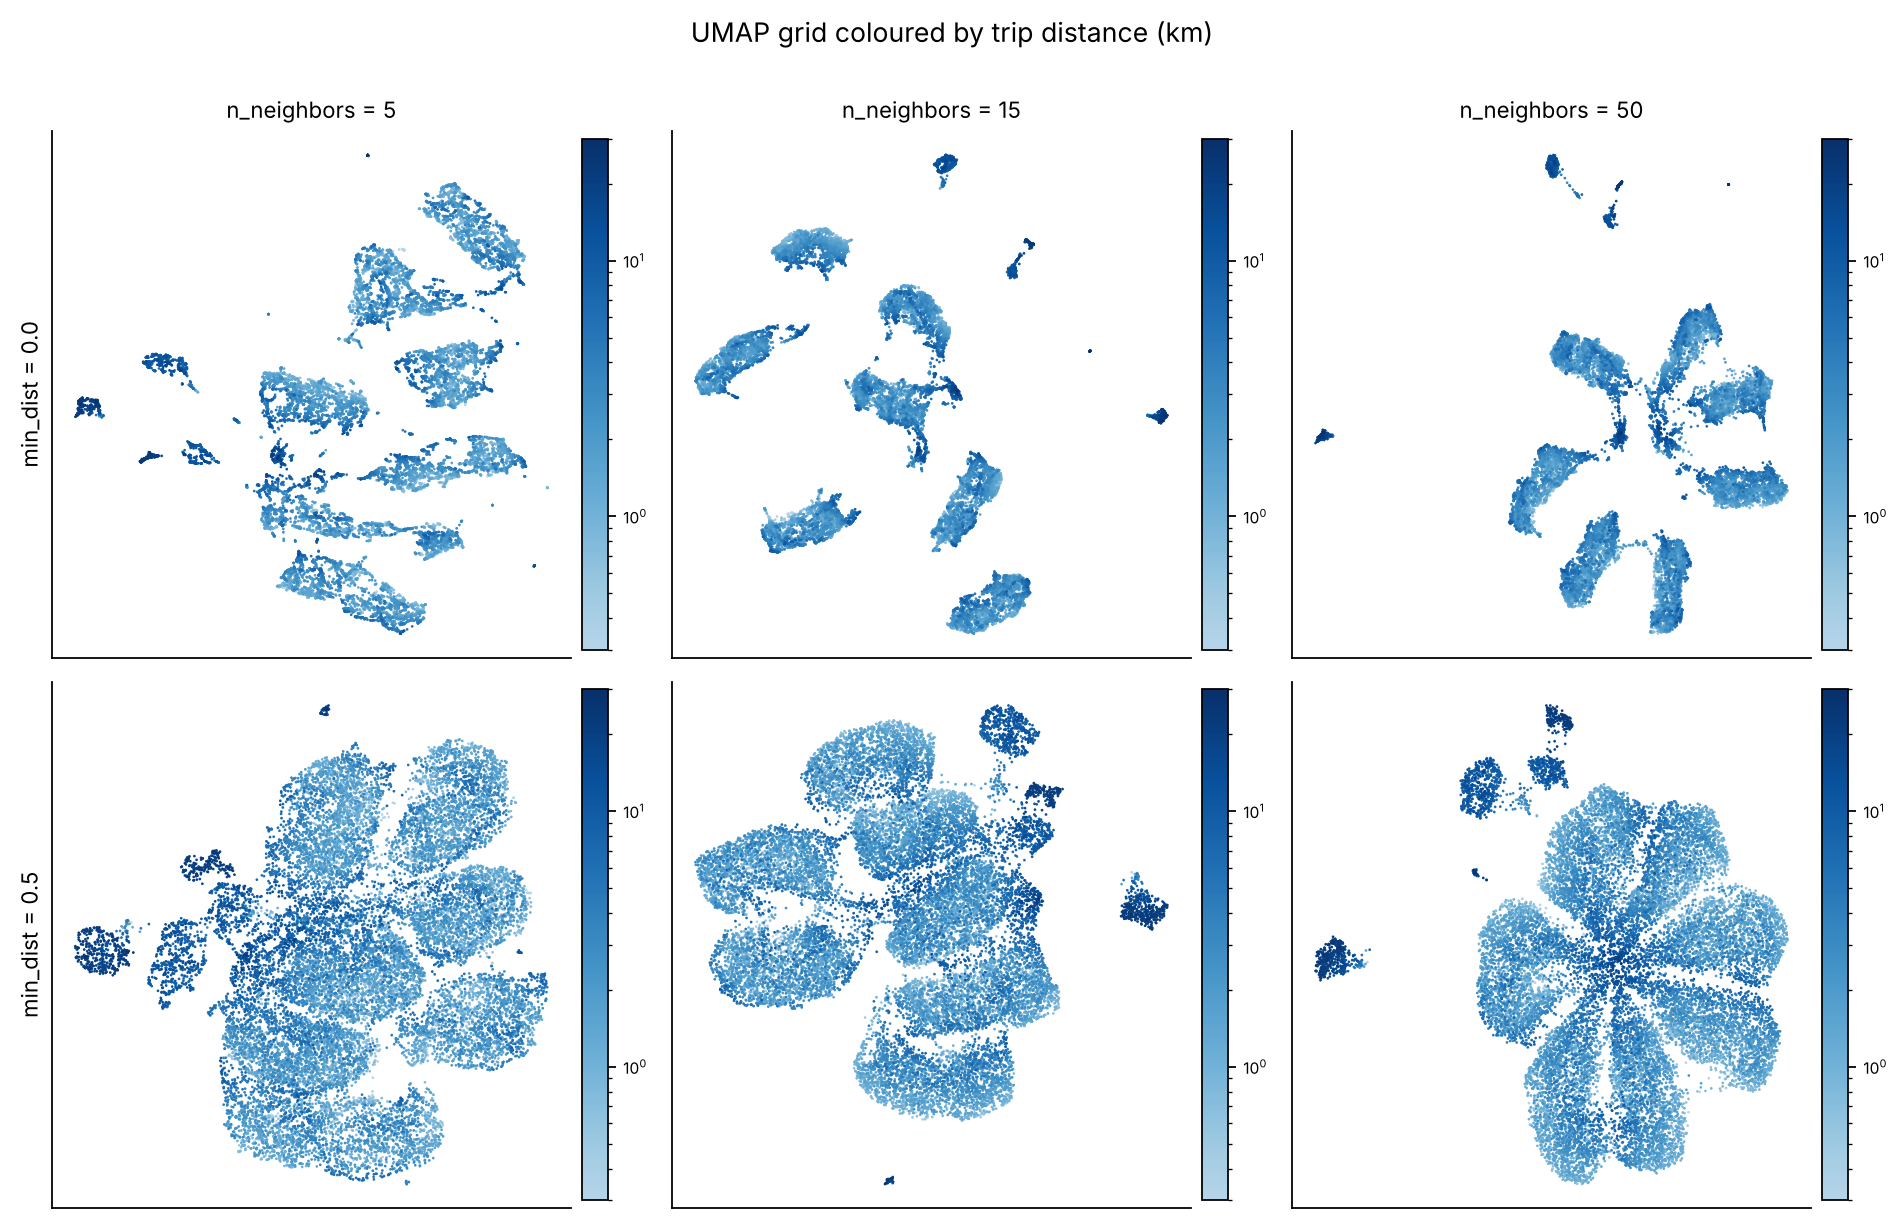
\includegraphics[width=0.62\linewidth]{section6_plots/q6_4_umap_grid_distance.png}\\[2pt]
  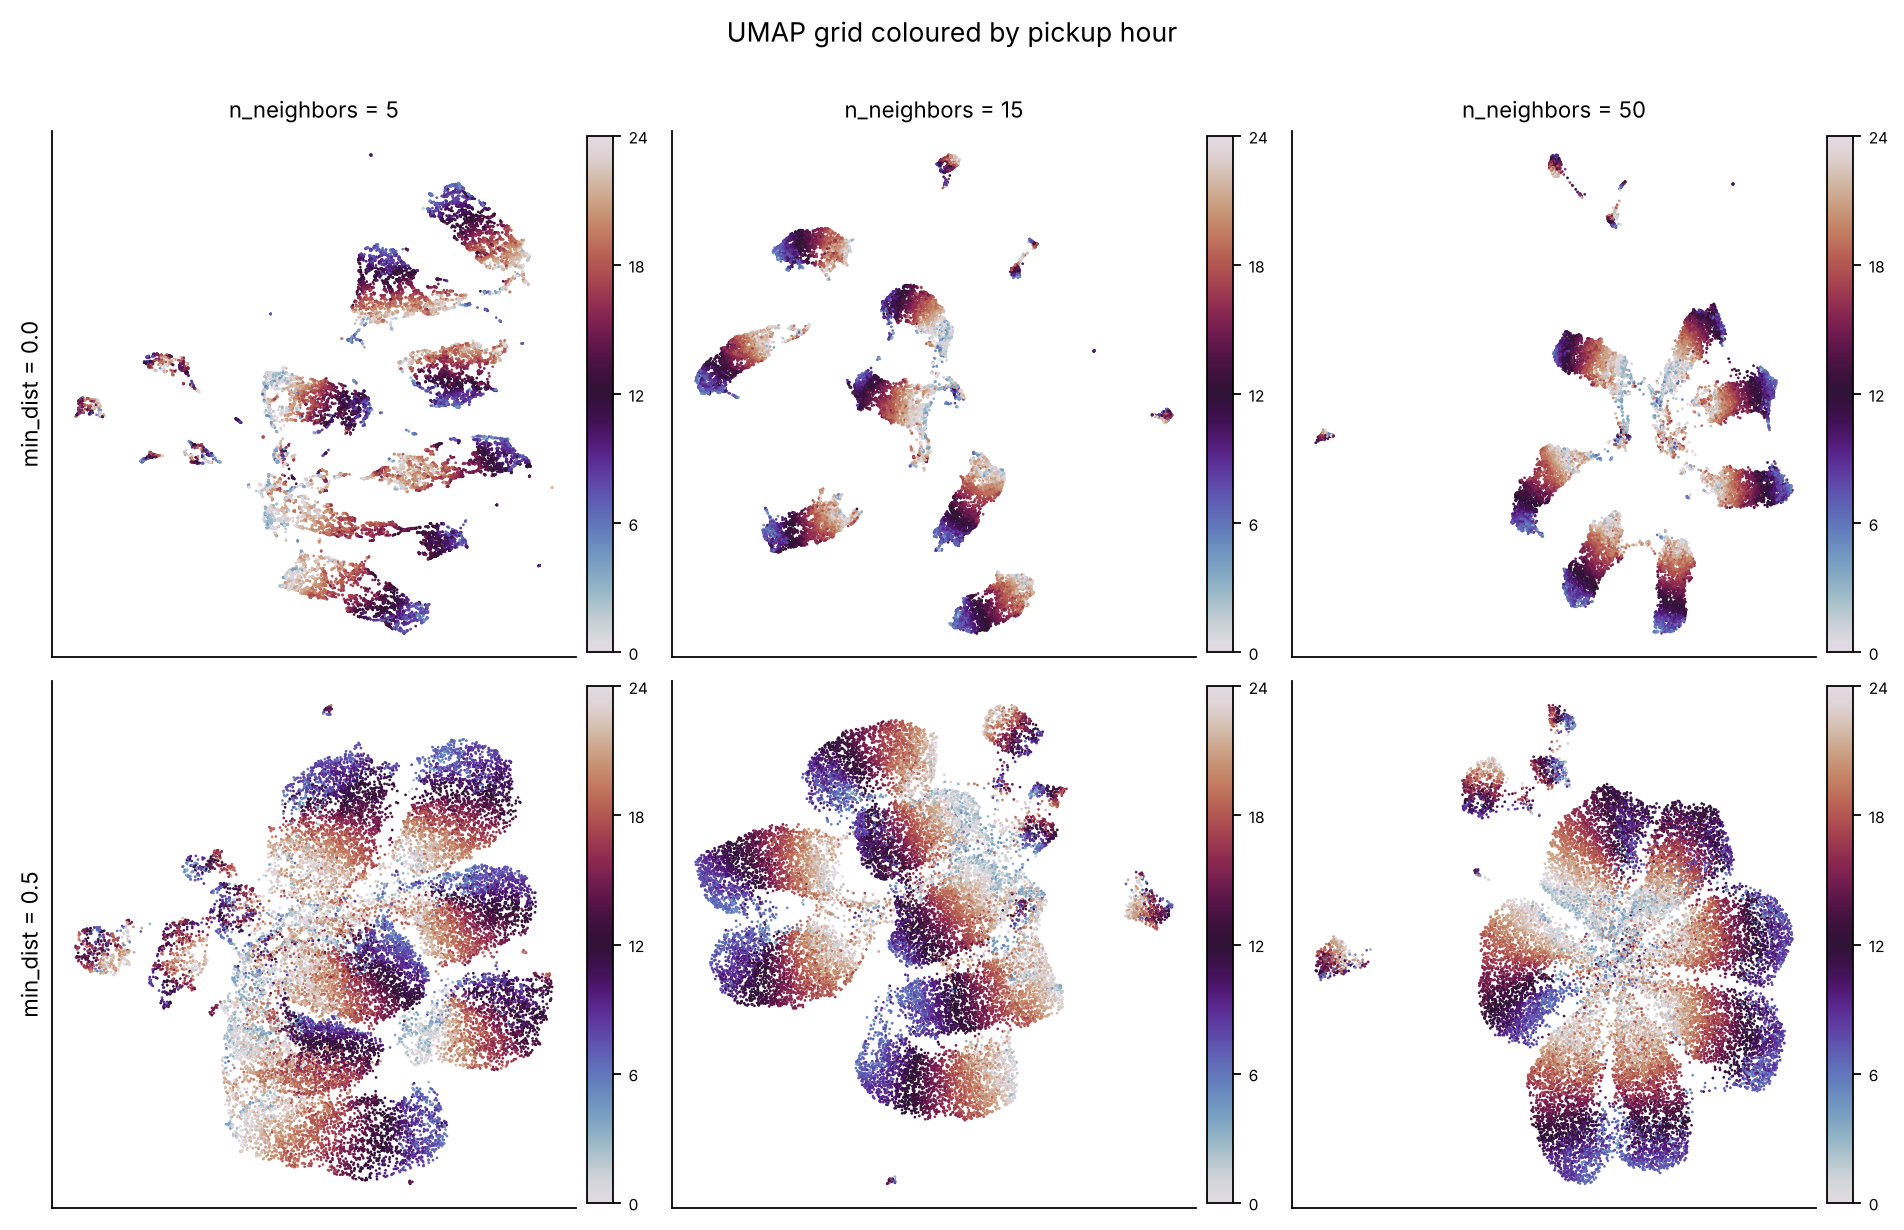
\includegraphics[width=0.49\linewidth]{section6_plots/q6_4_umap_grid_hour.png}\hfill
  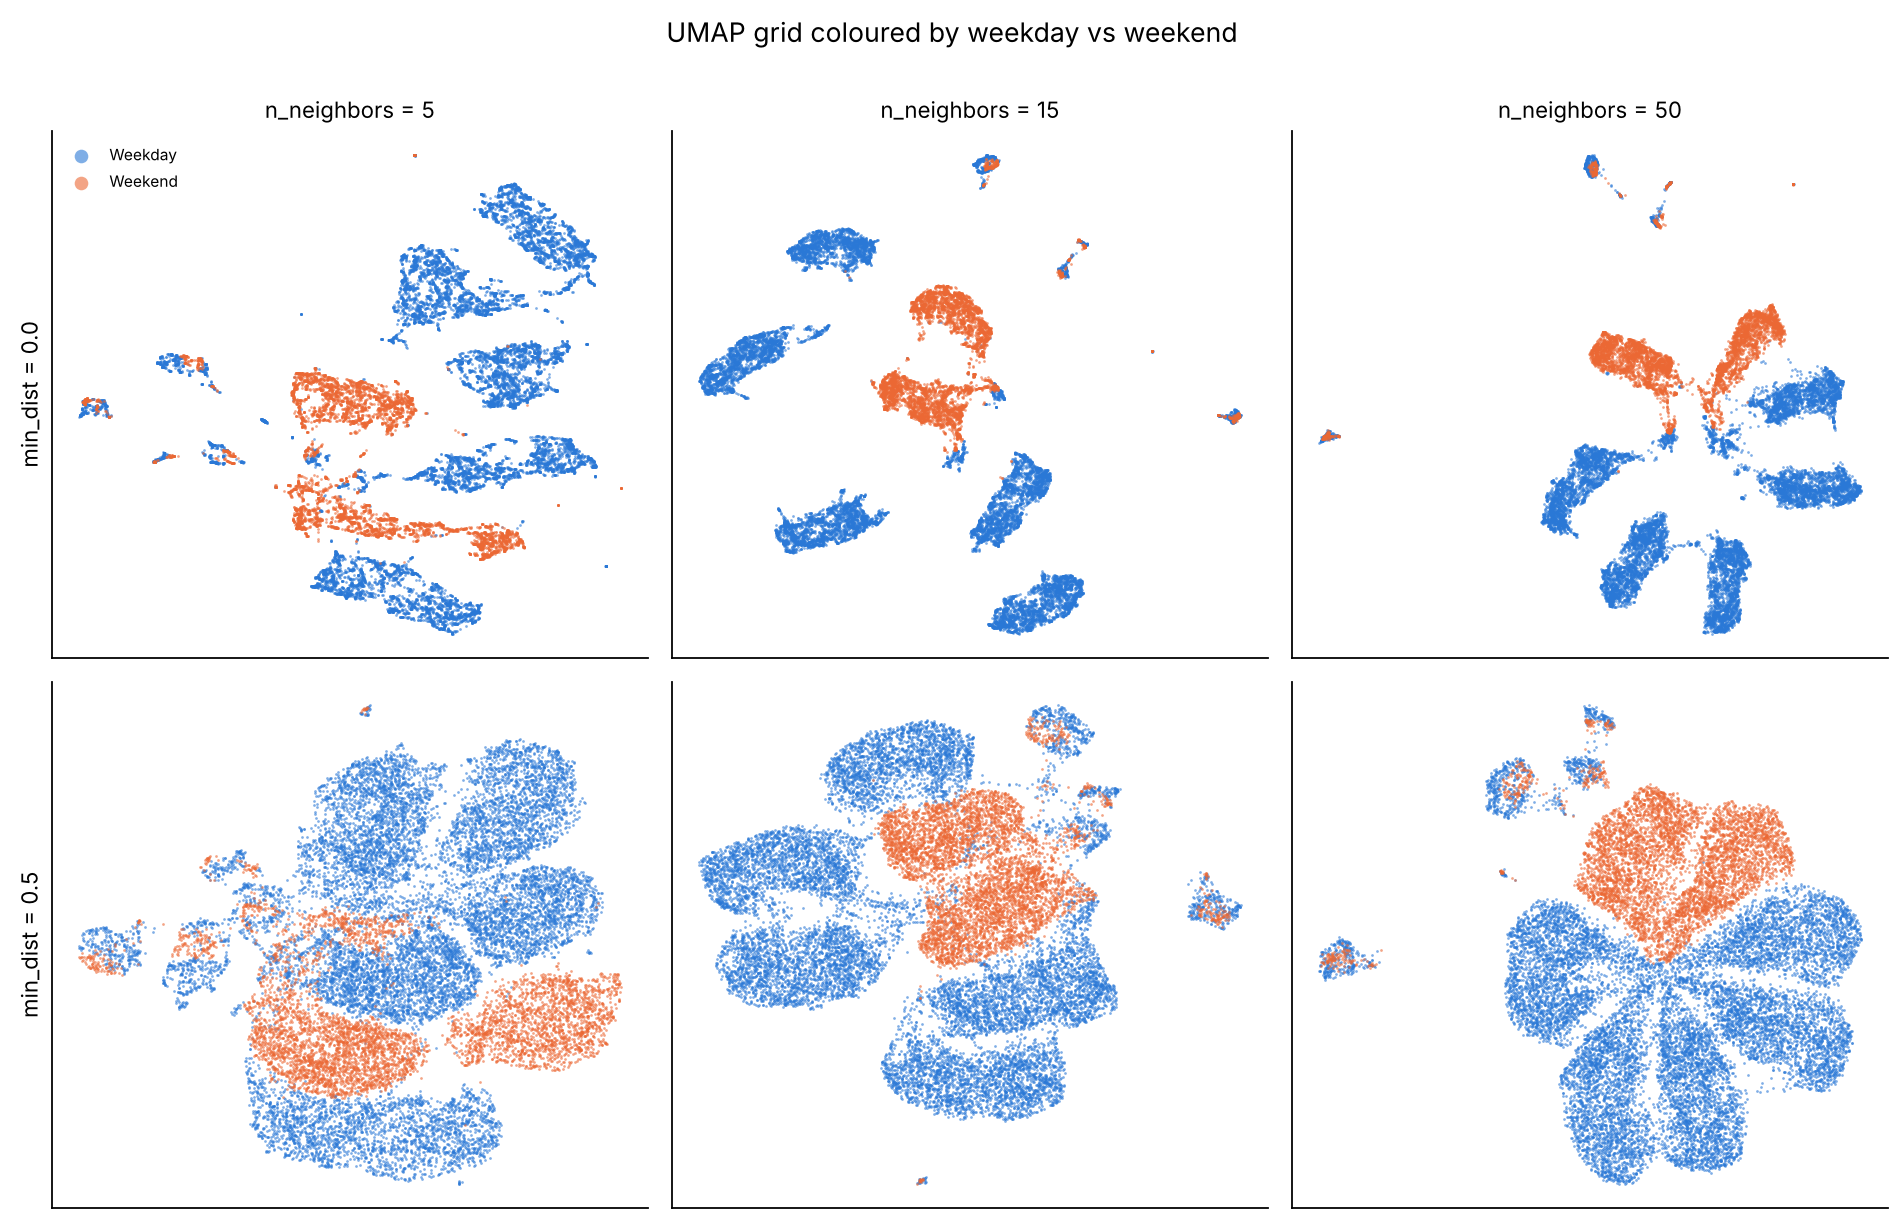
\includegraphics[width=0.49\linewidth]{section6_plots/q6_4_umap_grid_weekend.png}
  \caption{UMAP for \texttt{n\_neighbors} $\in\{5,15,50\}$ (columns of each grid) and \texttt{min\_dist} $\in\{0.0,0.5\}$ (rows), coloured by trip distance (top), pickup hour (bottom left) and weekday/weekend (bottom right).}
  \label{fig:q6_umap}
\end{figure}

In UMAP~\hyperref[ref:3]{[3]}, \textbf{\texttt{n\_neighbors}} plays the same role as perplexity (Figure~\ref{fig:q6_umap}). With 5 neighbours the map breaks into many thin fragments. With 50 it settles into seven large lobes plus a few small islands, and the global distance correlation improves from 0.319 to 0.461 (at \texttt{min\_dist} $=0$).

\textbf{\texttt{min\_dist}} only controls how tightly points are packed. At 0.0 the lobes are dense and separated by clear gaps, which suits density-based clustering. At 0.5 the points spread out, the gaps close and the lobes merge into a single flower shape. The structure underneath is the same, but it is harder to see where one group ends: trustworthiness drops from 0.964 to 0.928 at 50 neighbours.

In every setting the long trips (dark blue) separate from the rest. The hour and weekend colourings show that the seven lobes are days of the week, with hour as a gradient along each lobe. Section 6.6 returns to this. UMAP was much faster than t-SNE (6--24\,s per run; the first run also compiles the library and was the slowest).

\begin{table}[!htbp]
  \caption{Structure preserved by each 2D embedding, measured on a fixed random subset of 3{,}000 trips. Trustworthiness ($k=15$) measures local structure; Spearman $\rho$ between pairwise distances in the scaled feature space and in the embedding measures global structure. The best setting per method (highest mean) is in bold.}
  \label{tab:q6_scores}
  \centering
  \small
  \begin{tabular}{llccc}
    \toprule
    Method & Setting & Trustworthiness & Spearman $\rho$ & Mean \\
    \midrule
    PCA & PC1--PC2 & 0.758 & 0.766 & 0.762 \\
    \midrule
    t-SNE & perplexity 5 & 0.943 & 0.295 & 0.619 \\
    t-SNE & perplexity 30 & 0.971 & 0.313 & 0.642 \\
    t-SNE & \textbf{perplexity 100} & \textbf{0.978} & \textbf{0.357} & \textbf{0.667} \\
    \midrule
    UMAP & n=5, d=0.0 & 0.953 & 0.319 & 0.636 \\
    UMAP & n=15, d=0.0 & 0.960 & 0.368 & 0.664 \\
    UMAP & \textbf{n=50, d=0.0} & \textbf{0.964} & \textbf{0.461} & \textbf{0.713} \\
    UMAP & n=5, d=0.5 & 0.916 & 0.294 & 0.605 \\
    UMAP & n=15, d=0.5 & 0.929 & 0.353 & 0.641 \\
    UMAP & n=50, d=0.5 & 0.928 & 0.387 & 0.658 \\
    \bottomrule
  \end{tabular}
\end{table}

\textbf{Best embeddings.} We chose the setting with the highest mean of the two scores, so that neither local nor global structure is sacrificed: t-SNE with perplexity 100, and UMAP with \texttt{n\_neighbors}$=50$, \texttt{min\_dist}$=0.0$. These are used in the rest of the section.

\subsection*{6.5 Density-based clustering}

\textbf{Method and parameters.} DBSCAN~\hyperref[ref:1]{[1]} groups points that have at least \texttt{min\_samples} neighbours within a radius \texttt{eps} and labels the rest as noise. It was run on the eight principal components that explain 90\% of the variance, and on the best t-SNE and UMAP embeddings. \texttt{min\_samples} was fixed first. For PCA we used the usual heuristic of twice the dimension, $2\times8=16$. For the 2D embeddings that heuristic gives 4, which lets DBSCAN cut the dense embeddings into dozens of tiny clusters. We instead required 50 trips (0.25\% of the sample), the smallest group we would call a recurring trip type. \texttt{eps} was then read off the k-distance curve (distance to the $k$th neighbour, $k=$ \texttt{min\_samples}), at the knee: the point furthest from the straight line joining the ends of the sorted curve (Figure~\ref{fig:q6_kdist}).

\begin{figure}[!htbp]
  \centering
  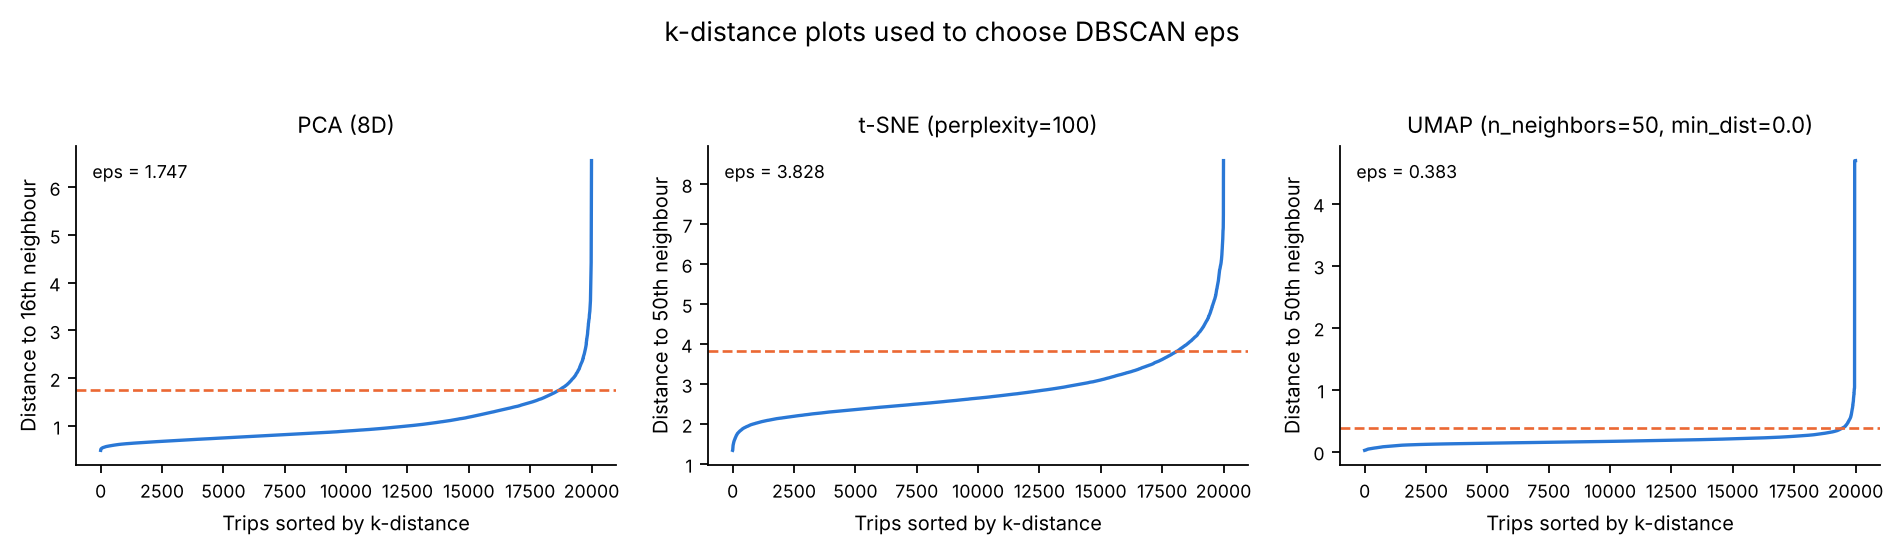
\includegraphics[width=0.8\linewidth]{section6_plots/q6_5_kdistance.png}
  \caption{Sorted k-distance curves. The dashed line is the knee used as \texttt{eps}.}
  \label{fig:q6_kdist}
\end{figure}

\begin{table}[!htbp]
  \caption{DBSCAN settings and results in each reduced space.}
  \label{tab:q6_dbscan}
  \centering
  \small
  \begin{tabular}{lcccc}
    \toprule
    Space & \texttt{min\_samples} & \texttt{eps} & Clusters & Noise \\
    \midrule
    PCA (8 components) & 16 & 1.747 & 3 & 2.2\% \\
    t-SNE (perplexity 100) & 50 & 3.828 & 10 & 1.1\% \\
    UMAP (n=50, d=0.0) & 50 & 0.383 & 13 & 0.8\% \\
    \bottomrule
  \end{tabular}
\end{table}

\begin{figure}[!htbp]
  \centering
  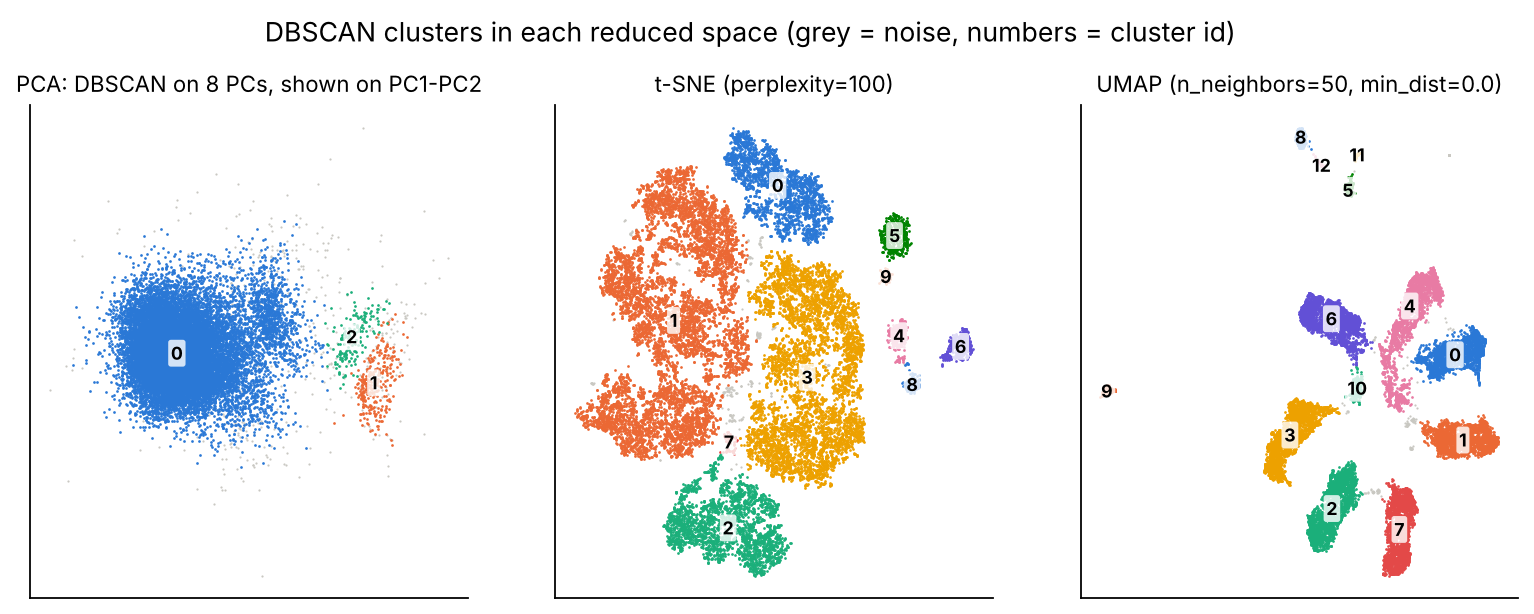
\includegraphics[width=0.85\linewidth]{section6_plots/q6_5_clusters.png}
  \caption{DBSCAN clusters. PCA clusters are found in eight dimensions and drawn on PC1--PC2. Grey points are noise; numbers are cluster ids, matching Table~\ref{tab:q6_profiles}.}
  \label{fig:q6_clusters}
\end{figure}

\textbf{Profiles and names.} Each cluster was profiled on the original, unscaled features (Table~\ref{tab:q6_profiles}). The airport columns use Section 5's flag, split by direction. Because several clusters were clearly LaGuardia trips, we also flagged pickups and drop-offs within 2\,km of LaGuardia (40.7769, $-73.8740$). This flag only describes clusters; it is not used as a feature or a filter. Names follow fixed rules: airport direction first, then day of week if one day makes up more than 80\% of the cluster, otherwise time of day, weekday/weekend, length and area.

\begin{table}[!htbp]
  \caption{Cluster profiles (original units; distance, duration and speed are medians). Hour is the circular mean pickup hour, used instead of the median because a plain median treats 23:00 and 00:00 as 23 hours apart. Wknd is the weekend share; Apt is the share of airport trips (Section 5 flag). Clusters are listed by size.}
  \label{tab:q6_profiles}
  \centering
  \scriptsize
  \setlength{\tabcolsep}{3.5pt}
  \begin{tabular}{llrrrrrrr}
    \toprule
    Space & Name (id) & Trips & Dist (km) & Dur (min) & Speed & Hour & Wknd & Apt \\
    \midrule
    PCA & evening all-week medium Manhattan trips (0) & 19,091 & 2.0 & 10.6 & 12.6 & 16:36 & 0.28 & 0.00 \\
     & JFK/Newark pickups to Manhattan (1) & 294 & 20.3 & 43.6 & 26.9 & 17:57 & 0.28 & 0.98 \\
     & Manhattan rides to JFK/Newark (2) & 171 & 20.4 & 41.3 & 29.2 & 11:58 & 0.30 & 0.90 \\
    \midrule
    t-SNE & evening weekday medium Manhattan trips (1) & 7,958 & 1.9 & 10.7 & 11.6 & 16:12 & 0.01 & 0.00 \\
     & evening weekend medium Manhattan trips (3) & 5,607 & 2.2 & 10.1 & 14.3 & 18:36 & 0.93 & 0.00 \\
     & Friday Manhattan trips (2) & 2,586 & 1.8 & 10.2 & 11.0 & 16:36 & 0.00 & 0.00 \\
     & Monday Manhattan trips (0) & 2,105 & 1.7 & 9.1 & 12.1 & 15:26 & 0.00 & 0.00 \\
     & LaGuardia pickups to Manhattan (5) & 513 & 9.8 & 30.7 & 20.2 & 16:35 & 0.25 & 0.00 \\
     & JFK/Newark pickups to Manhattan (6) & 411 & 19.9 & 39.1 & 27.0 & 18:01 & 0.28 & 0.97 \\
     & Manhattan rides to LaGuardia (4) & 292 & 9.8 & 26.9 & 22.3 & 11:02 & 0.28 & 0.00 \\
     & Manhattan rides to JFK/Newark (8) & 197 & 20.3 & 39.9 & 30.5 & 12:05 & 0.29 & 0.84 \\
     & late-night Friday Manhattan trips (7) & 62 & 1.7 & 3.6 & 27.9 & 04:58 & 0.00 & 0.00 \\
     & LaGuardia pickups to Queens (9) & 50 & 3.2 & 13.3 & 14.6 & 12:40 & 0.24 & 0.00 \\
    \midrule
    UMAP & Sunday Manhattan trips (4) & 2,896 & 2.4 & 10.5 & 15.0 & 19:36 & 0.86 & 0.00 \\
     & Friday Manhattan trips (3) & 2,728 & 1.8 & 10.1 & 11.3 & 16:44 & 0.00 & 0.00 \\
     & Saturday Manhattan trips (6) & 2,672 & 2.0 & 9.8 & 12.8 & 17:58 & 0.99 & 0.00 \\
     & Thursday Manhattan trips (2) & 2,641 & 1.8 & 10.4 & 11.2 & 15:44 & 0.00 & 0.00 \\
     & Wednesday Manhattan trips (7) & 2,497 & 1.8 & 10.1 & 11.3 & 15:35 & 0.00 & 0.00 \\
     & Tuesday Manhattan trips (1) & 2,393 & 1.8 & 10.1 & 11.4 & 15:11 & 0.00 & 0.00 \\
     & Monday Manhattan trips (0) & 2,256 & 1.8 & 9.3 & 12.5 & 15:23 & 0.00 & 0.00 \\
     & LaGuardia pickups to Manhattan (8) & 516 & 9.8 & 30.3 & 20.2 & 16:34 & 0.25 & 0.00 \\
     & JFK/Newark pickups to Manhattan (9) & 411 & 19.9 & 39.1 & 27.0 & 18:01 & 0.28 & 0.97 \\
     & Manhattan rides to LaGuardia (5) & 300 & 9.9 & 26.7 & 22.7 & 11:10 & 0.28 & 0.00 \\
     & late-night all-week long Manhattan trips (10) & 294 & 10.5 & 20.2 & 30.5 & 00:49 & 0.43 & 0.00 \\
     & Manhattan rides to JFK/Newark (11) & 188 & 20.3 & 40.5 & 30.4 & 11:49 & 0.30 & 0.88 \\
     & LaGuardia pickups to Queens (12) & 53 & 3.1 & 12.8 & 15.0 & 12:13 & 0.24 & 0.00 \\
    \bottomrule
  \end{tabular}
\end{table}

The three spaces tell one consistent story about the long trips and three different stories about everything else.
\begin{itemize}
  \item \textbf{PCA} finds only three groups. One holds 95\% of trips (Manhattan trips at all times: median 2.0\,km and 10.6\,min). The other two are \emph{JFK/Newark pickups to Manhattan} (294 trips) and \emph{Manhattan rides to JFK/Newark} (171 trips), both about 20\,km and 40--45\,min.
  \item \textbf{t-SNE} finds the same two airport runs (411 and 197 trips), adds two LaGuardia runs (513 into Manhattan, 292 out to LaGuardia) and a small \emph{LaGuardia pickups to Queens} group of short local trips. It splits the large Manhattan mass into weekday (7{,}958) and weekend (5{,}607) groups, with separate Friday and Monday lobes. It also finds a 62-trip \emph{late-night Friday Manhattan trips} cluster: very short (3.6\,min), fast (28\,km/h) trips with a mean pickup time near 05:00.
  \item \textbf{UMAP} finds all of the airport and LaGuardia runs again, plus a \emph{late-night long trip} group: 294 trips with a mean pickup hour around 01:00, 10\,km and 30\,km/h. It splits the Manhattan mass into seven clusters, \textbf{one for each day of the week} (each over 99\% one day, except Sunday at 83\%).
\end{itemize}
The pickup maps (Figures~\ref{fig:q6_maps_umap} and~\ref{fig:q6_maps_other}) make the difference visible. The seven day clusters cover exactly the same part of Manhattan, while the airport and LaGuardia clusters pick up at the airport or drop off in Midtown. This matches Section 4, where LaGuardia and JFK are the only strong pickup concentrations outside Manhattan in the heatmaps, and LaGuardia hosts the largest Thursday-evening hotspot.

\begin{figure}[!htbp]
  \centering
  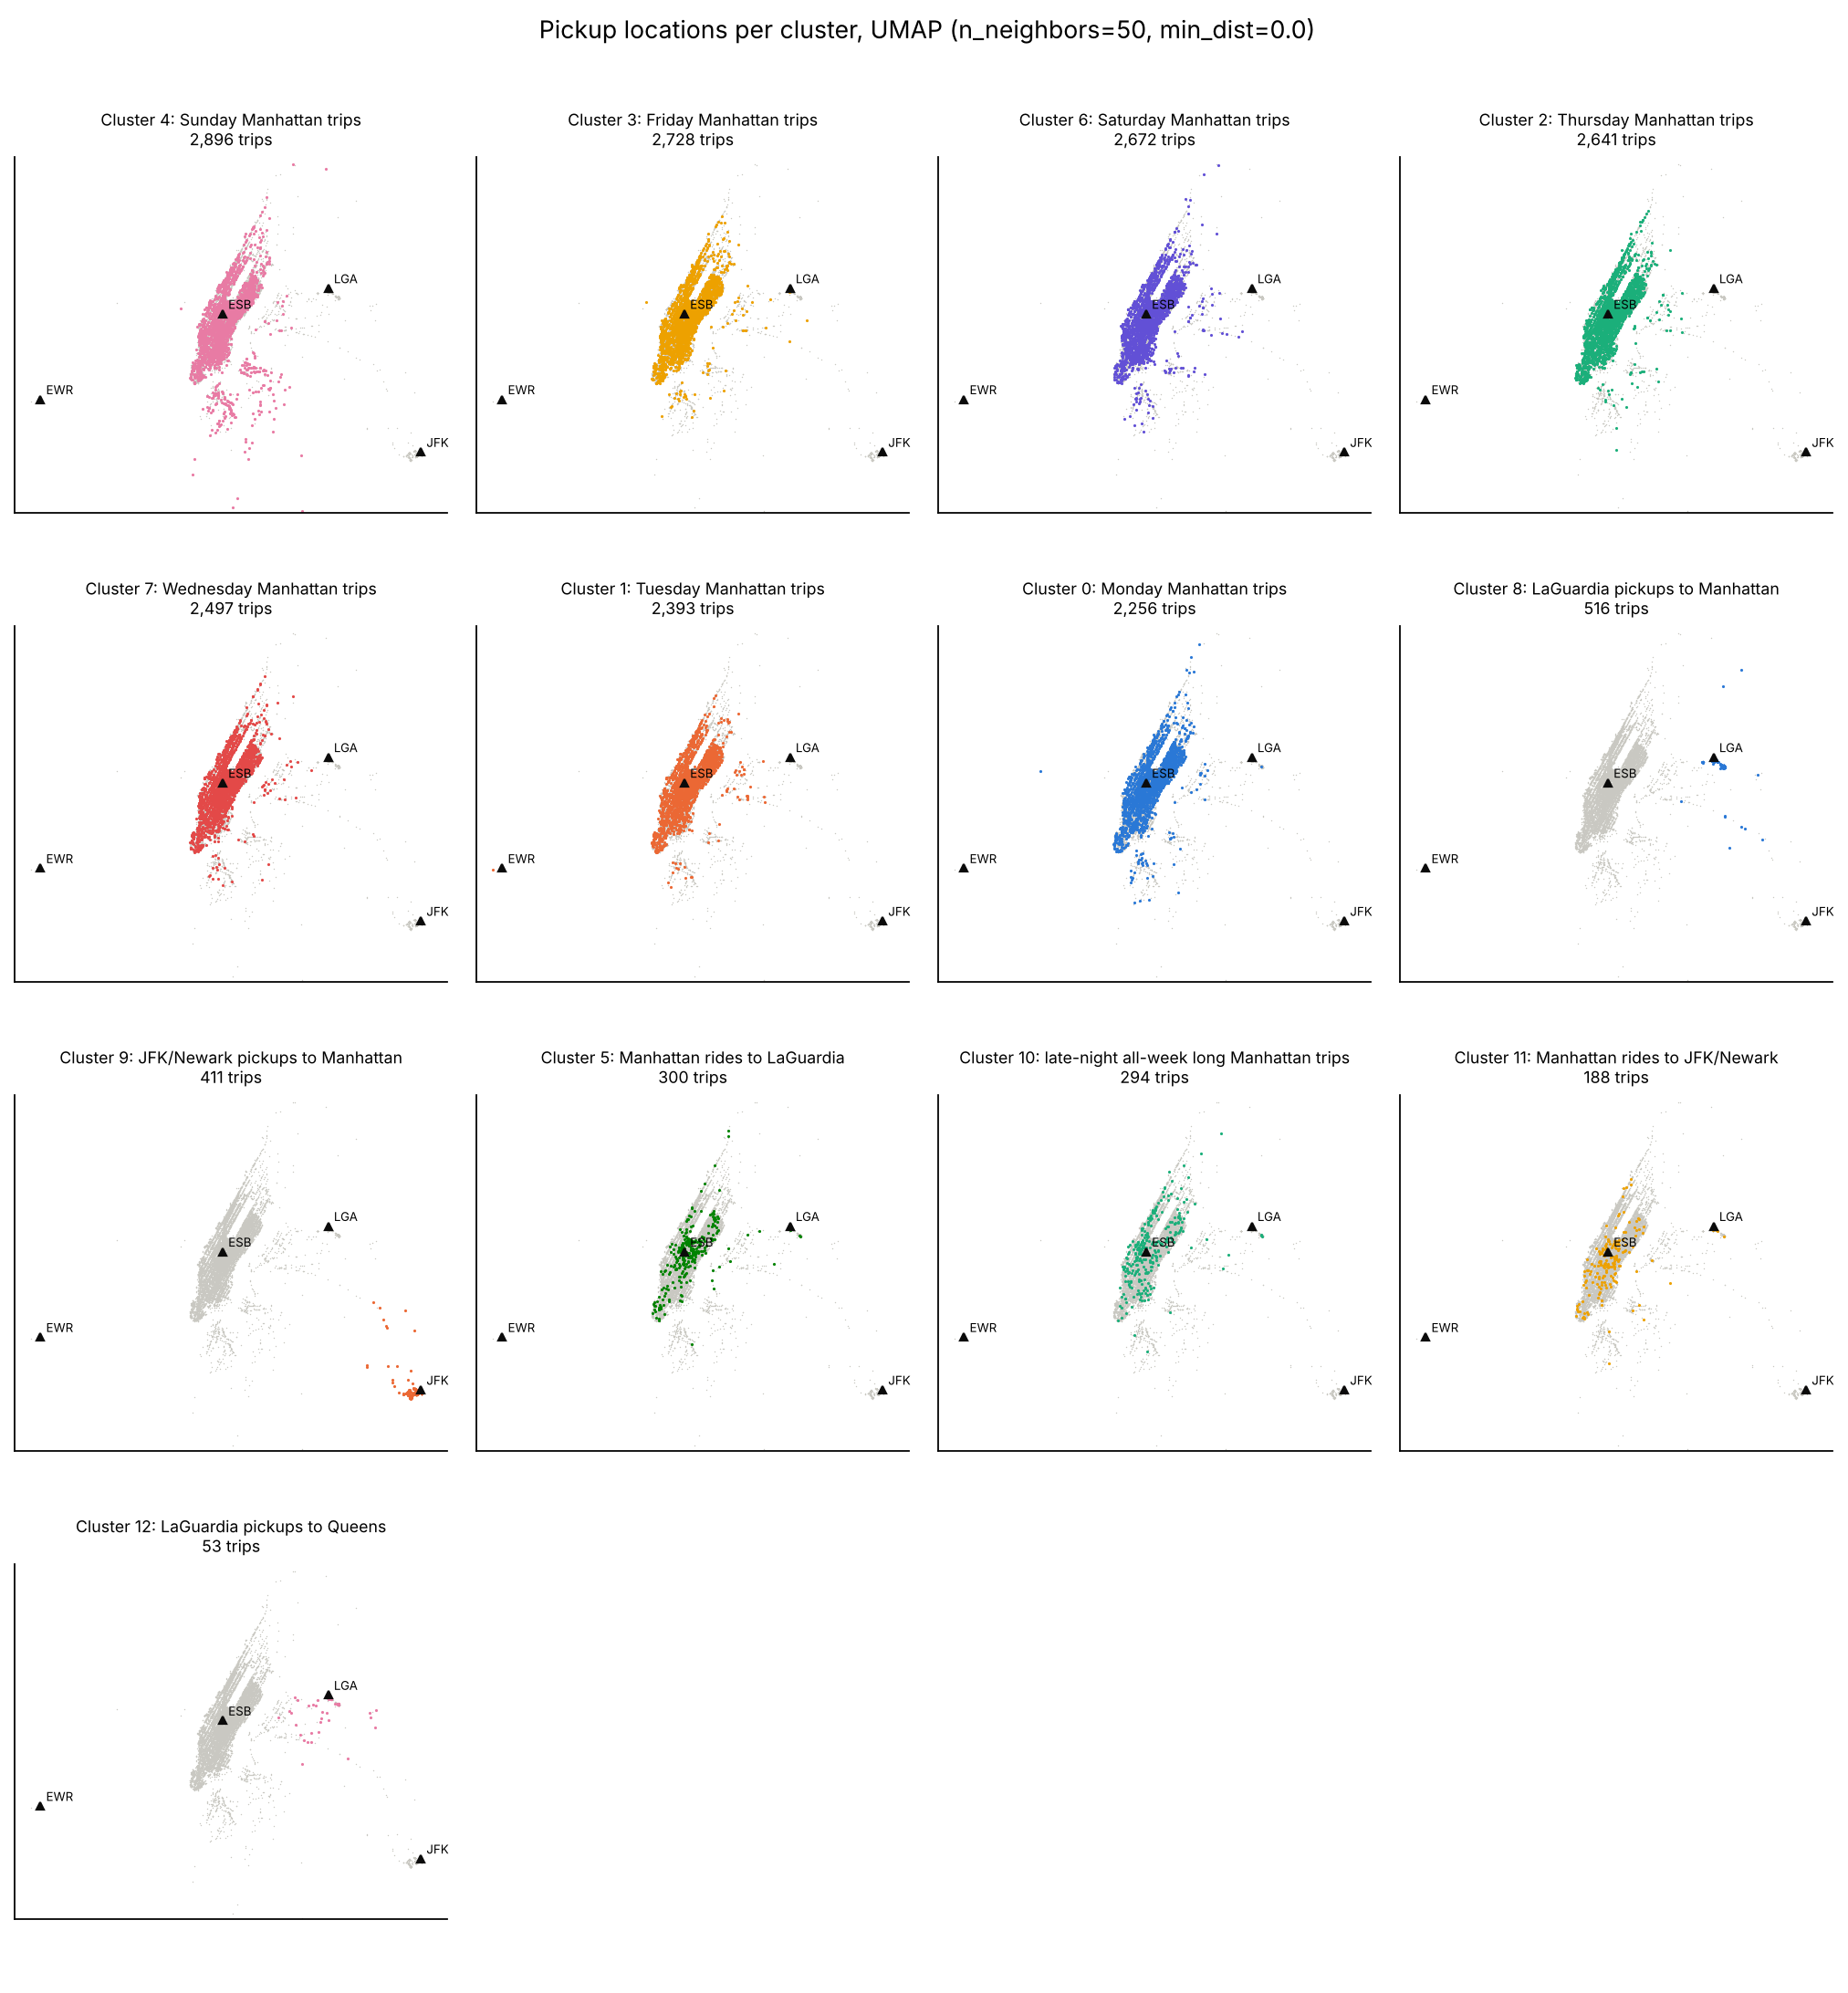
\includegraphics[width=0.66\linewidth]{section6_plots/q6_5_maps_umap.png}
  \caption{Pickup locations of each UMAP cluster (colour) against all sampled pickups (grey).}
  \label{fig:q6_maps_umap}
\end{figure}

\begin{figure}[!htbp]
  \centering
  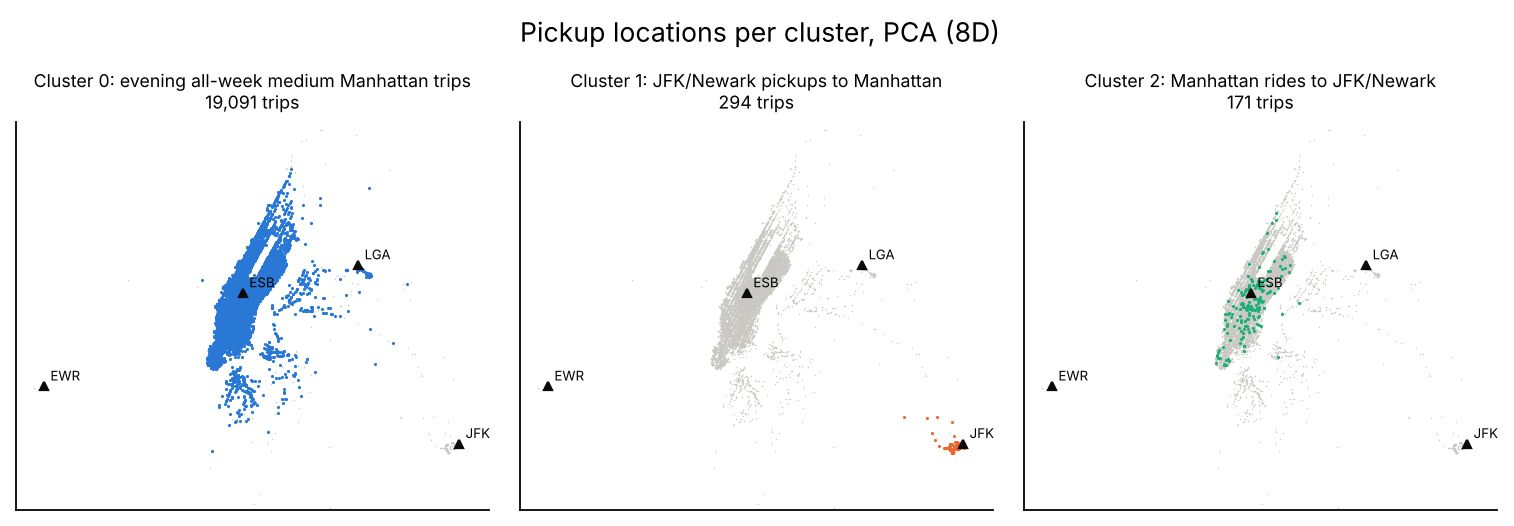
\includegraphics[width=0.45\linewidth]{section6_plots/q6_5_maps_pca.png}\\[2pt]
  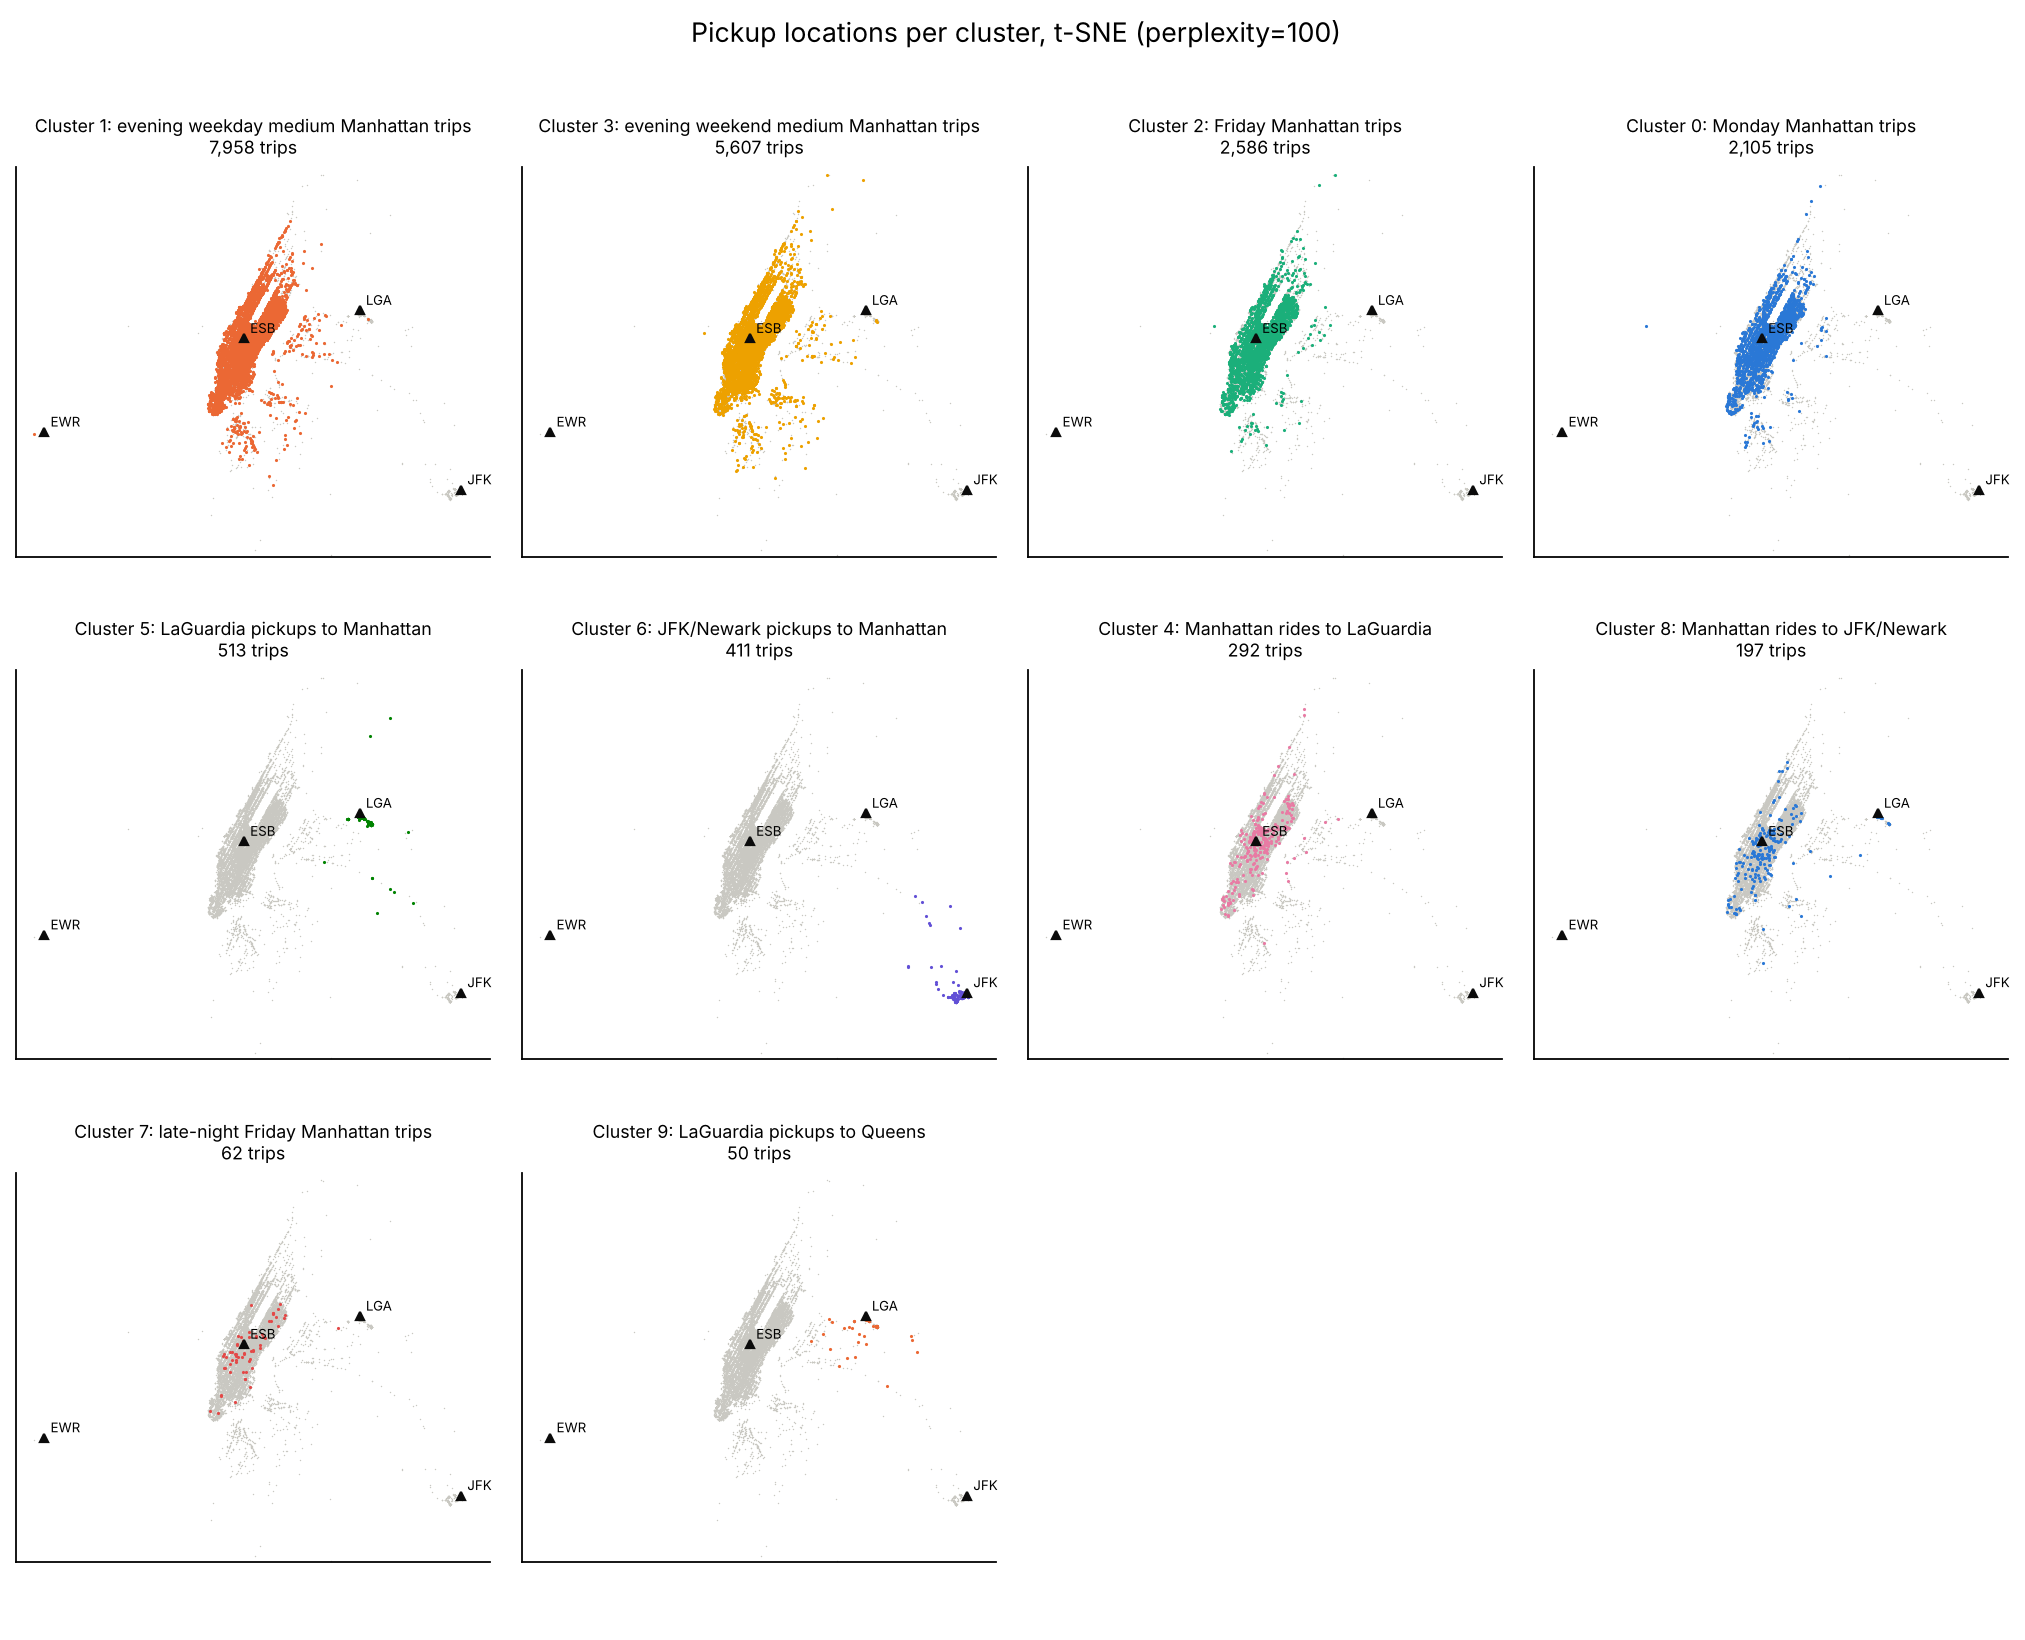
\includegraphics[width=0.6\linewidth]{section6_plots/q6_5_maps_tsne.png}
  \caption{Pickup locations of each PCA cluster (top) and each t-SNE cluster (bottom).}
  \label{fig:q6_maps_other}
\end{figure}

\subsection*{6.6 Comparison}

\begin{figure}[!htbp]
  \centering
  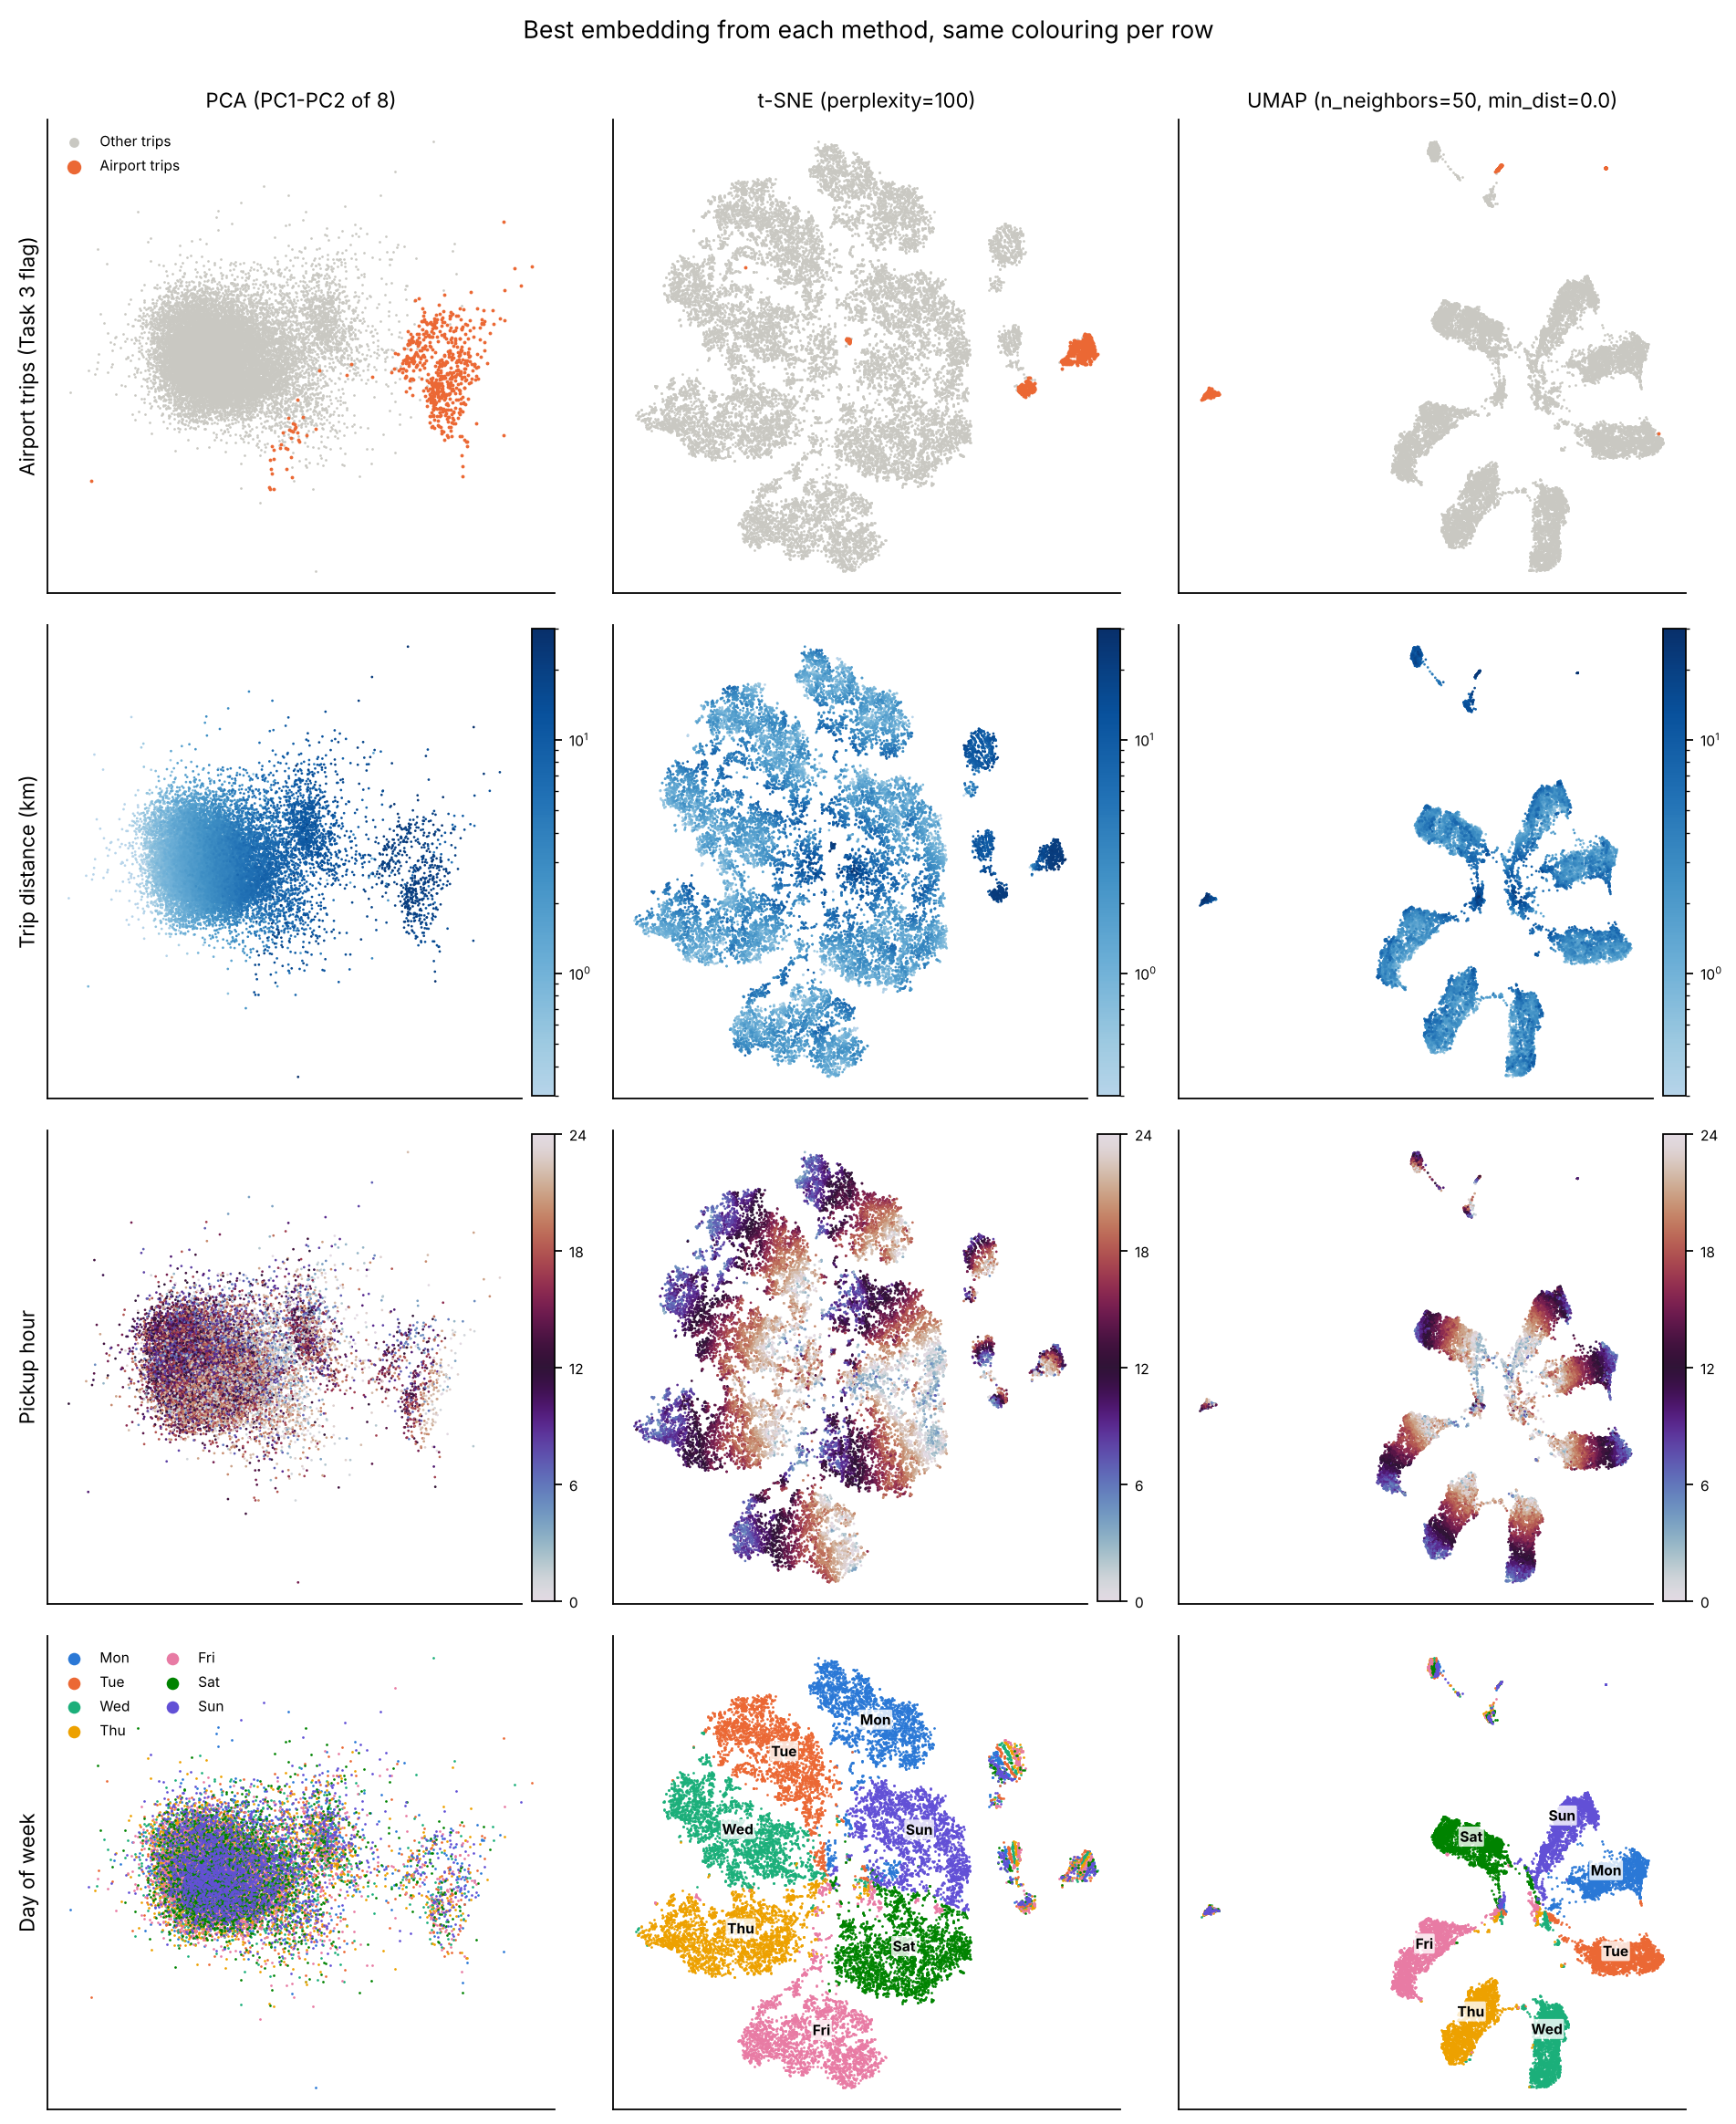
\includegraphics[width=0.68\linewidth]{section6_plots/q6_6_side_by_side.png}
  \caption{Best embedding per method (columns) with the same colouring in each row: Section 5 airport flag, distance, pickup hour and day of week.}
  \label{fig:q6_side}
\end{figure}

\textbf{Groups that appear in all three methods.} Airport trips form their own group in every method (Figure~\ref{fig:q6_side}, top row). Of the 598 airport trips in the sample, 66.6\% fall in a single JFK/Newark-to-Manhattan cluster in both t-SNE and UMAP, and that cluster is 96.8\% airport trips. PCA also isolates them (98.3\% pure), but it sends 26.1\% of the airport trips to noise, against 5.5\% for t-SNE and UMAP. Direction matters: trips \emph{from} the airport and trips \emph{to} the airport form separate clusters in every space, because pickup and drop-off coordinates are separate features. These long-trip groups, together with LaGuardia runs in t-SNE and UMAP, are the only structure all three methods agree on.

\textbf{What PCA reveals and misses.} PCA gives axes with a meaning (trip length and north--south location) and keeps global distances best ($\rho=0.766$). It shows that most trips form one continuum rather than separate types. Because it is linear and keeps only two of the eight important directions in the plot, it misses everything carried by time: hour and day are invisible on PC1--PC2, and in eight dimensions DBSCAN still sees a single main cloud. Its local structure is the weakest (trustworthiness 0.758). The non-linear methods recover the time structure that PCA spreads across PC3--PC6.

\textbf{Local and global structure.} t-SNE and UMAP preserve neighbourhoods well (trustworthiness 0.978 and 0.964) but global distances poorly ($\rho=0.357$ and $0.461$). Within a lobe, nearby points really are similar trips. Distances \emph{between} lobes, the empty space separating them and the area each lobe covers cannot be read as similarity or size. t-SNE in particular equalises density, so a small, tight group of airport runs and a large diffuse group of Manhattan trips can end up looking alike. UMAP keeps somewhat more of the global layout (the airport islands sit far from Manhattan, as they should), but its gaps are still not to scale. Only in PCA are distances and spreads directly interpretable.

\textbf{The day-of-week structure.} The bottom row of Figure~\ref{fig:q6_side} shows that the seven UMAP lobes, and most t-SNE lobes, are days of the week. Day of week takes only seven values, so after the cyclic encoding every day sits at its own fixed point on a circle. Adjacent days are 1.22 apart in scaled units, more than the median distance from a trip to its nearest neighbour (0.59) or even its 15th-nearest neighbour (1.08). Each day therefore becomes a separate shelf of the data. Methods built on nearest neighbours turn these shelves into islands. The agreement between clusters and day of week, measured by ARI, is 0.83 for UMAP, 0.45 for t-SNE and 0.00 for PCA. As a check we reran the chosen UMAP without the two day-of-week columns (Figure~\ref{fig:q6_nodow}). The lobes disappear, and DBSCAN with the same rule finds six clusters: one main Manhattan mass (18{,}266 trips), the four airport and LaGuardia runs, and a late-night group of long Manhattan-to-Queens trips (148 trips, mean pickup hour about 00:00). The ARI against the original UMAP clusters is only 0.045.

\begin{figure}[!htbp]
  \centering
  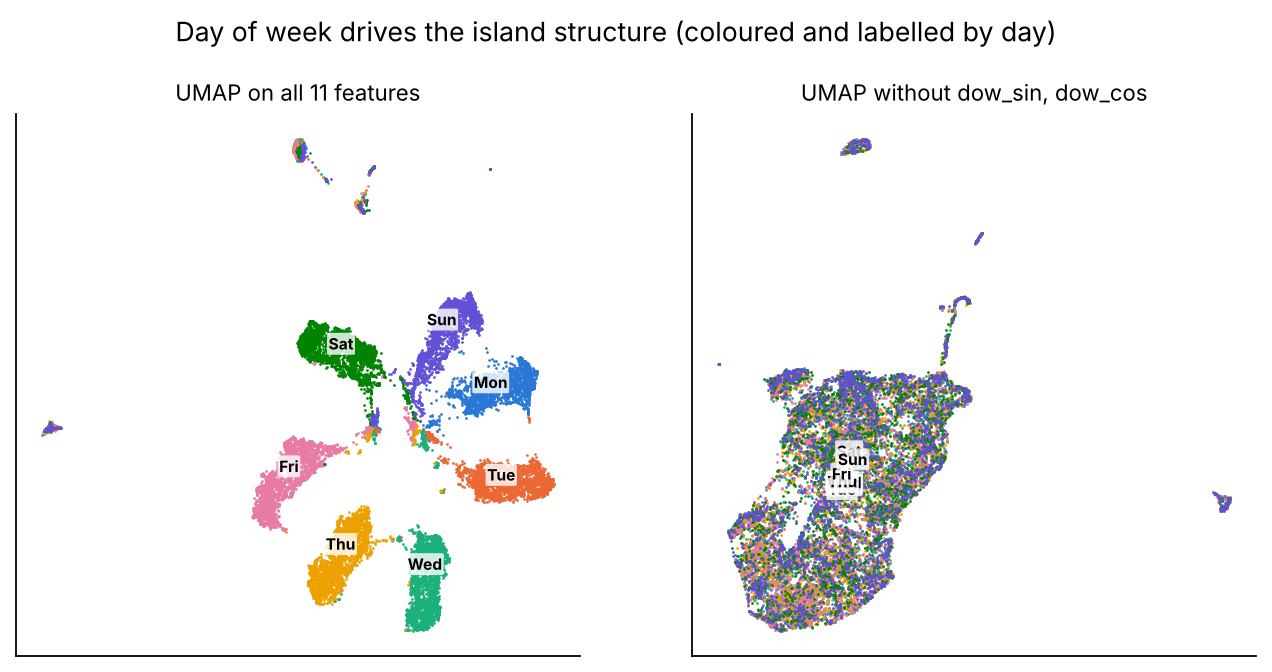
\includegraphics[width=0.6\linewidth]{section6_plots/q6_6_umap_without_dow.png}
  \caption{The chosen UMAP on all eleven features (left) and without \texttt{dow\_sin}/\texttt{dow\_cos} (right), coloured by day of week.}
  \label{fig:q6_nodow}
\end{figure}

\textbf{Runtime and sensitivity.} On the same 2-core machine, PCA takes a fraction of a second, has no tuning parameters and gives the same answer for any seed. UMAP takes 6--24\,s per run and t-SNE 86--161\,s, growing with perplexity. Both non-linear methods change markedly with their main parameter (Figures~\ref{fig:q6_tsne} and~\ref{fig:q6_umap}). To test the seed, we reran the chosen settings with seeds 0 and 7 and compared each run with seed 42 (Table~\ref{tab:q6_seeds}). With PCA initialisation, t-SNE returned exactly the same embedding for all three seeds (Procrustes disparity 0, identical neighbours). In scikit-learn the seed only enters through the initial layout, and PCA initialisation fixes that layout. With random initialisation the layout changed (disparity 0.10--0.13, and 74--76\% of each trip's 15 neighbours kept), and DBSCAN found between 8 and 12 clusters (ARI 0.61--0.76 against seed 42). UMAP changed most at the level of individual neighbours: only 41--43\% of neighbours were kept, with disparity 0.11--0.33. Its clusters were fairly stable, though (9 to 11 clusters against 13, ARI 0.71--0.80). In every run the airport and LaGuardia islands reappear, while some of the day lobes merge or split. PCA has no seed dependence.

\begin{table}[!htbp]
  \caption{Seed sensitivity of the chosen settings, comparing seeds 0 and 7 with seed 42. Procrustes disparity is 0 for identical layouts up to rotation and scale. kNN overlap is the mean share of each trip's 15 nearest embedding neighbours that are the same across seeds. ARI compares DBSCAN clusters found with the same rule.}
  \label{tab:q6_seeds}
  \centering
  \small
  \begin{tabular}{llcccc}
    \toprule
    Method & Seed & Procrustes & kNN overlap & Clusters & ARI vs seed 42 \\
    \midrule
    t-SNE & 0 & 0.000 & 1.000 & 10 & 1.000 \\
    t-SNE & 7 & 0.000 & 1.000 & 10 & 1.000 \\
    t-SNE (random init) & 0 & 0.102 & 0.757 & 12 & 0.612 \\
    t-SNE (random init) & 7 & 0.132 & 0.735 & 8 & 0.761 \\
    UMAP & 0 & 0.111 & 0.433 & 11 & 0.800 \\
    UMAP & 7 & 0.328 & 0.409 & 9 & 0.710 \\
    \bottomrule
  \end{tabular}
\end{table}

\textbf{Agreement between methods.} Table~\ref{tab:q6_ari} gives the adjusted Rand index between each pair of clusterings. We handle noise in two ways: treating noise as one extra label (all points), and keeping only trips that both methods assign to a cluster.

\begin{table}[!htbp]
  \caption{Adjusted Rand index between cluster labels.}
  \label{tab:q6_ari}
  \centering
  \small
  \begin{tabular}{lccc}
    \toprule
    Pair & ARI, noise as a label & ARI, clustered in both & Share clustered in both \\
    \midrule
    PCA vs t-SNE & 0.054 & 0.037 & 97.0\% \\
    PCA vs UMAP & 0.021 & 0.014 & 97.2\% \\
    t-SNE vs UMAP & 0.480 & 0.490 & 98.3\% \\
    \bottomrule
  \end{tabular}
\end{table}

Agreement is low with PCA and moderate between t-SNE and UMAP. The two ways of handling noise give almost the same values, because all methods label very few trips as noise. ARI is dominated by how the large Manhattan mass is divided: PCA keeps it whole, t-SNE splits it mainly into weekday and weekend, and UMAP into seven days. The small airport and LaGuardia clusters, which match closely across methods, barely move the index. A low ARI therefore does not mean the methods disagree about everything. It means they disagree about the part of the data that has no clear clusters.

\textbf{Can t-SNE and UMAP clusters be trusted?} Partly. We checked each clustering in the original 11-dimensional space by asking how many of a trip's 15 nearest neighbours there share its cluster. The answer is 0.970 for t-SNE and 0.957 for UMAP, against chance levels of 0.272 and 0.121. So the clusters are not invented by the projection: they are coherent regions of the feature space. Coherent is not the same as natural, though. The day-of-week clusters are coherent only because we put day of week into the feature matrix, and they disappear once those two columns are removed. Clusters found in an embedding are hypotheses that must be checked against the original features and against other methods. Here the airport and LaGuardia runs pass every check, while the day-of-week clusters reflect our encoding rather than the trips.

\textbf{Recommendation.} For exploring this dataset we recommend \textbf{UMAP} (\texttt{n\_neighbors}$=50$, \texttt{min\_dist}$=0.0$), used together with PCA. UMAP had the best balance of local and global structure in Table~\ref{tab:q6_scores}, recovered every group the other methods found, and ran many times faster than t-SNE, which makes it practical to try several feature sets and parameters. PCA should sit beside it because its axes can be interpreted and its distances can be trusted, which keeps us from reading too much into UMAP's islands. t-SNE produced similar groups but was the slowest and is no more interpretable. Whatever the method, clusters should be named and checked from profiles in the original units, as in Table~\ref{tab:q6_profiles}. The analysis also suggests treating day of week as a colouring or a filter rather than a feature when the goal is to find trip types.

\section*{References}
{\small
\begin{itemize}
  \setlength{\itemsep}{4pt}

  \item[{[1]}]\phantomsection\label{ref:1} M.~Ester, H.-P.~Kriegel, J.~Sander, and X.~Xu.
    A Density-Based Algorithm for Discovering Clusters in Large Spatial Databases with Noise.
    In \textit{Proceedings of the Second International Conference on Knowledge Discovery and Data Mining (KDD-96)},
    pages 226--231, 1996.
    \url{https://www.osti.gov/biblio/421283}

  \item[{[2]}]\phantomsection\label{ref:2} L.~van der Maaten and G.~Hinton.
    Visualizing Data using t-SNE.
    \textit{Journal of Machine Learning Research}, 9(86):2579--2605, 2008.
    \url{https://jmlr.org/papers/v9/vandermaaten08a.html}

  \item[{[3]}]\phantomsection\label{ref:3} L.~McInnes, J.~Healy, and J.~Melville.
    UMAP: Uniform Manifold Approximation and Projection for Dimension Reduction.
    \textit{arXiv preprint arXiv:1802.03426}, 2018.
    \url{https://arxiv.org/abs/1802.03426}
\end{itemize}
}

\end{document}